\documentclass[12pt,titlepage]{article}
\usepackage[margin=1in]{geometry}
\usepackage{graphicx,amsmath,blindtext,minted}
\usepackage{hyperref}
\hypersetup{
    colorlinks,
    citecolor=black,
    filecolor=black,
    linkcolor=black,
    urlcolor=black
}
\usepackage{caption,subcaption}

%% Variables definition
\newcommand{\vSubject}{Basic Programming Practicum}
\newcommand{\vSubtitle}{Final Exam Project}
\newcommand{\vName}{Dicha Zelianivan Arkana}
\newcommand{\vNIM}{2241720002}
\newcommand{\vClass}{1i}
\newcommand{\vDepartment}{Information Technology}
\newcommand{\vStudyProgram}{D4 Informatics Engineering}

%% [START] Tikz related stuff
\usepackage{tikz}
\usetikzlibrary{svg.path,calc,shapes.geometric,shapes.misc}
\tikzstyle{terminator} = [rectangle, draw, text centered, rounded corners = 1em, minimum height=2em]
\tikzstyle{preparation} = [chamfered rectangle, chamfered rectangle sep=0.75em, draw, text centered, minimum height = 2em]
\tikzstyle{process} = [rectangle, draw, text centered, minimum height=2em]
\tikzstyle{decision} = [diamond, aspect=2, draw, text centered, minimum height=2em]
\tikzstyle{data}=[trapezium, draw, text centered, trapezium left angle=60, trapezium right angle=120, minimum height=2em]
\tikzstyle{connector} = [line width=0.25mm,->]
%% [END] Tikz related stuff

%% [START] Fancy header related stuff
\usepackage{fancyhdr}
\pagestyle{fancy}
\setlength{\headheight}{15pt} % compensate fancyhdr style
\fancyhead{}
\fancyfoot{}
\fancyfoot[L]{\thepage}
\fancyfoot[R]{\textit{\vSubject - \vSubtitle}}
\renewcommand{\footrulewidth}{0.4pt}% default is 0pt, overline for footer
%% [END] Fancy header related stuff

%% [START] Custom tabular command related stuff
\usepackage{tabularx}
\newcommand{\details}[2]{
    #1 & #2  \\
}
%% [END] Custom tabular command related stuff

%% [START] Figure related stuff
\newcommand{\image}[3][1]{
    \begin{figure}[h]
        \centering
        \includegraphics[#1]{#2}
        \caption{#3}
        \label{#3}
    \end{figure}
}
%% [END] Figure related stuff

\begin{document}
\begin{titlepage}
    \centering
    \vfill
    {\bfseries\LARGE
        \vSubject\\
        \vskip0.25cm
        \vSubtitle\\
    }
    \vskip0.25cm
    \bfseries\Large{Students Code of Conduct Management System}
    \vfill
    
\includegraphics[width=6cm]{images/polinema-logo.png}
    \vfill
    {
        \textbf{Name}\\
        \vName\\
        \vskip0.5cm
        \textbf{NIM}\\
        \vNIM\\
        \vskip0.5cm
        \textbf{Class}\\
        \vClass\\
        \vskip0.5cm
        \textbf{Department}\\
        \vDepartment\\
        \vskip0.5cm
        \textbf{Study Program}\\
        \vStudyProgram
    }
\end{titlepage}

\tableofcontents
\pagebreak
\listoffigures
\pagebreak

\section{Preliminary}
This document provides the documentation of how to use a CLI app that keep track of Student's violated rules.
It includes a detailed steps on how to use each and every menu, a flowchart to understand the code flow, and the code itself.

\section{Compiling and Running}
The app itself is just a single \texttt{.java} file so it should be trivial to run it. It can be compiled using the \texttt{javac} command
and then use the \texttt{java} command to run it.

Although, the app is provided in a form of Maven project, so it would be easier to just use an Integrated Development Environment (IDE) and import the project itself.
After doing that, simply press \texttt{Ctrl + F5} or the play button in the IDE.

For a better experience, the app should be run on a terminal that supports ANSI escape code, such as the new Windows Terminal,
because the program uses \texttt{\symbol{92}033[H\symbol{92}033[2J} to reset the screen state.
It is done to simulate how a page navigation would work inside a GUI app.

\section{Usage}
These are the steps to use each and every part that is available on the app, including the logic behind it.

\subsection{Top Level Menu}
\subsubsection{Logging In}
Upon running the app, there should be a prompt asking the user to log in. Since there is no database integration, the credential is hardcoded.
Insert \textbf{admin} as the username and \textbf{admin123} as the password.

\begin{figure}[h]
    \centering
    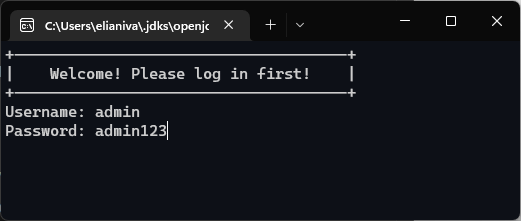
\includegraphics[width=.7\textwidth]{images/login.png}
    \caption{The app prompting a username and password}
\end{figure}

\subsubsection{Main Menu}
After the user logged in, there should be a main menu with a greeting message. The greeting message will only appear on initial login.
It will not appear later on.

\begin{figure}[h]
    \centering
    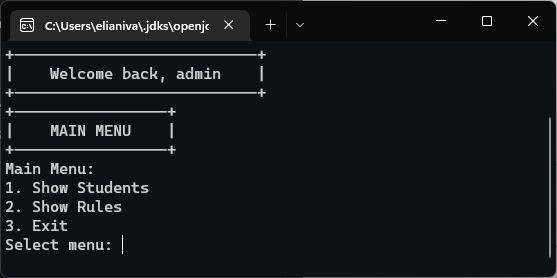
\includegraphics[width=.8\textwidth]{images/main-menu.png}
    \caption{The app showing a main menu}
\end{figure}

\subsection{Students Menu}
On the main menu, choose the first menu to show a list of actions related to Student operations.
The app should now display all students along with their menu.

\begin{figure}[h]
    \centering
    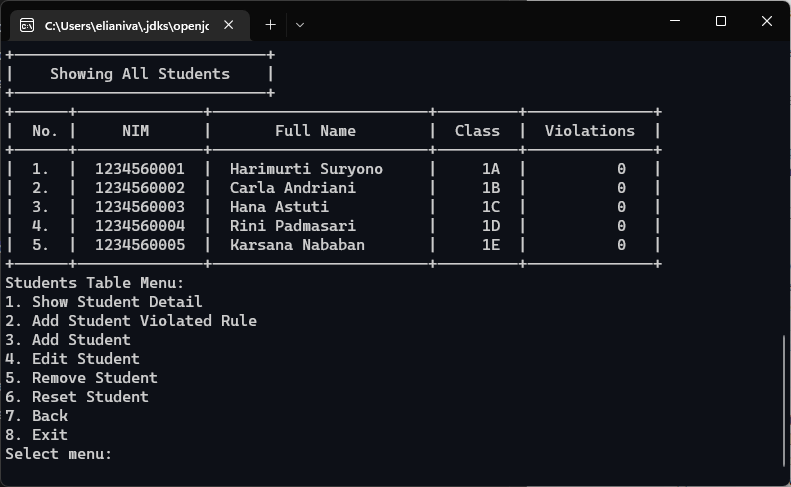
\includegraphics[width=.8\textwidth]{images/student-menu.png}
    \caption{The app showing students list along with their menu}
\end{figure}

\subsubsection{Student Entity}
Before going with the rest of the menu, there are some things that should be noted.
These are some details regarding each Student entity along with its validation

\begin{enumerate}
    \item {
        \textbf{NIM}
        \begin{itemize}
            \item Min Length: 10 characters
            \item Max Length: 10 characters
            \item Allowed to be empty: No
        \end{itemize}
    }
    \item {
        \textbf{Full Name}
        \begin{itemize}
            \item Min Length: 1 character
            \item Max Length: 20 characters
            \item Allowed to be empty: No
        \end{itemize}
    }
    \item {
        \textbf{Class}
        \begin{itemize}
            \item Min Length: 1 character
            \item Max Length: 2 characters
            \item Allowed to be empty: No
        \end{itemize}
    }
    \item {
        \textbf{Violated Rules}
        \begin{itemize}
            \item Min Length: 0 character
            \item Max Length: 3 characters
            \item Allowed to be empty: Yes
        \end{itemize}
    }
    \item {
        \textbf{Total Violations}
        \begin{itemize}
            \item Min: 0
            \item Max: \texttt{Integer.MAX\_VALUE}
            \item Allowed to be empty: No, but has a default value of 0
        \end{itemize}
    }
\end{enumerate}

\pagebreak

\subsubsection{Adding Violated Rule to a Student}
The main purpose of this app is to manage rules that have been violated by the student along with its punishment.
To do this, select the \textbf{Add Student Violated Rule}. Upon selecting the menu, the app will prompt for a student's NIM.

\begin{figure}[h]
    \centering
    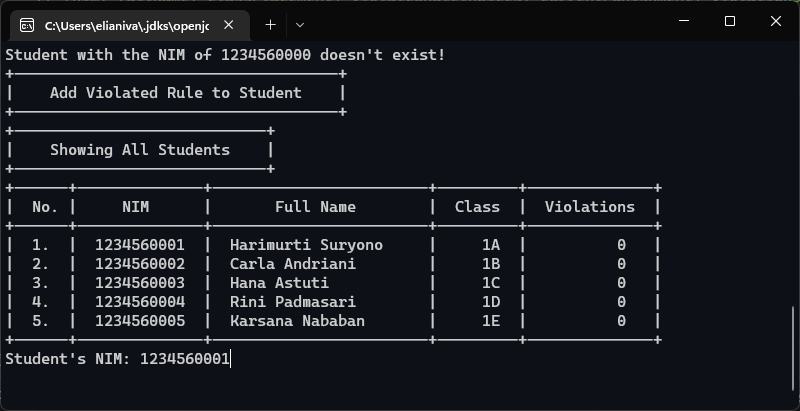
\includegraphics[width=.8\textwidth]{images/add-student-rule-input.png}
    \caption{The app asking for student's NIM and showing a warning when student was not found}
\end{figure}

After successfuly selcting the student, the app will show the list of the rules and ask for a rule id to be attached to the student
indicating that the student has violated that rule. The same input validation applies.

\begin{figure}[h]
    \centering
    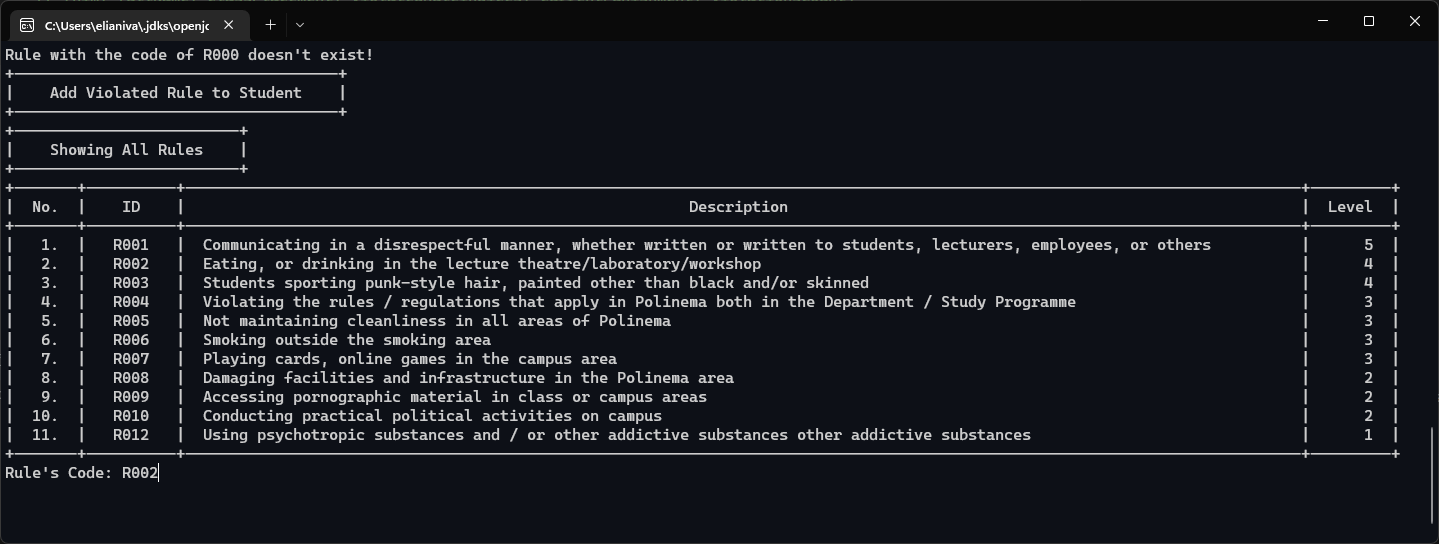
\includegraphics[width=.8\textwidth]{images/add-student-rule-input-2.png}
    \caption{The app asking for rule's id and showing a warning when student was not found}
\end{figure}

\pagebreak

The app should show the success message after attaching the rule to the student

\begin{figure}[h]
    \centering
    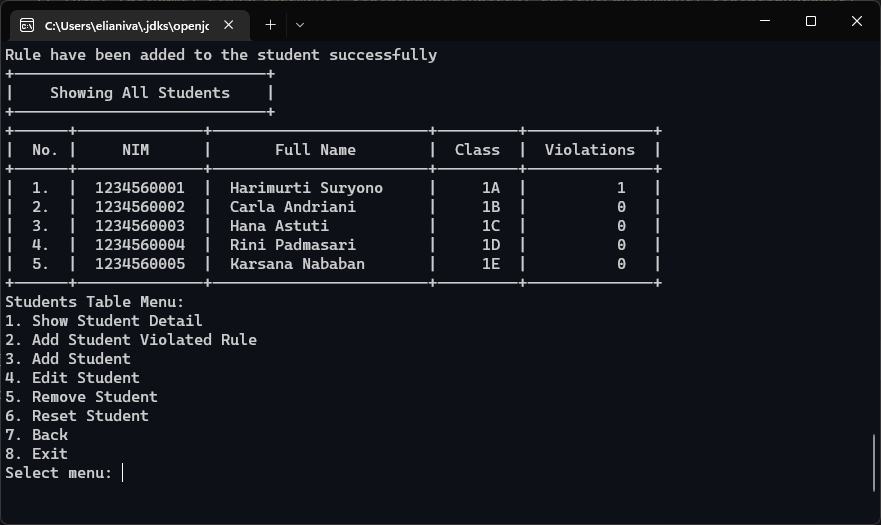
\includegraphics[width=.8\textwidth]{images/add-student-rule-success.png}
    \caption{The app showing a success message}
\end{figure}

If the student has maxed out the limit, meaning that they have violated 3 rules and haven't done
the punishment that is given, then the app will throw an error.

\begin{figure}[h]
    \centering
    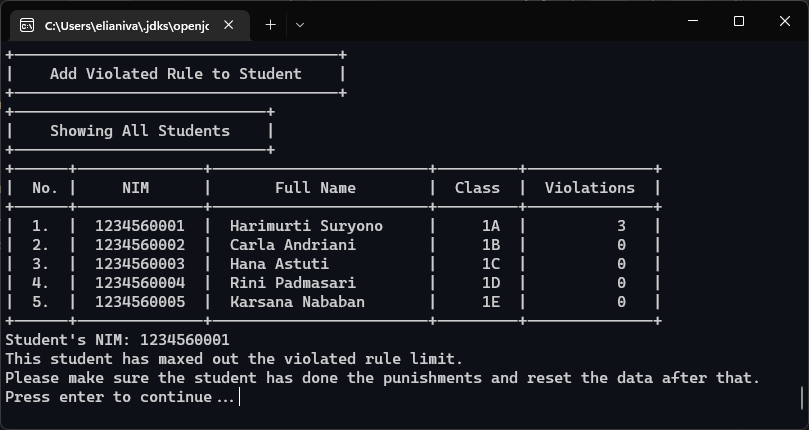
\includegraphics[width=.8\textwidth]{images/add-student-rule-max.png}
    \caption{The app showing an error because it maxed out}
\end{figure}

\pagebreak

Here are some brief rules regarding the rules:
\begin{itemize}
    \item If the student has 3 rules, new rule can't be added. The student need to be reset first.
    \item If the student received 3 rules on the same level, the next punishment is going to be the punishment for the next level.
\end{itemize}

\subsubsection{Showing a Student Detail}
To show a student detail, simply select the \textbf{Show Student Detail} menu and the app will prompt for a student NIM.

\begin{figure}[h]
    \centering
    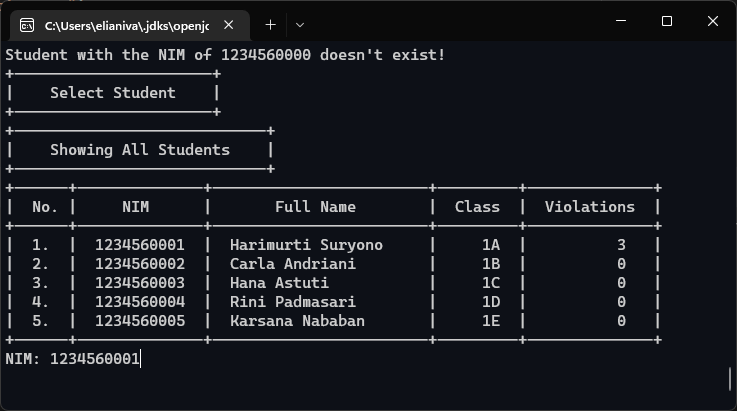
\includegraphics[width=.8\textwidth]{images/show-student-input.png}
    \caption{The app asking for a Student NIM}
\end{figure}

The student detail shows their detail along with their violated rules and punishments.

\begin{figure}[h]
    \centering
    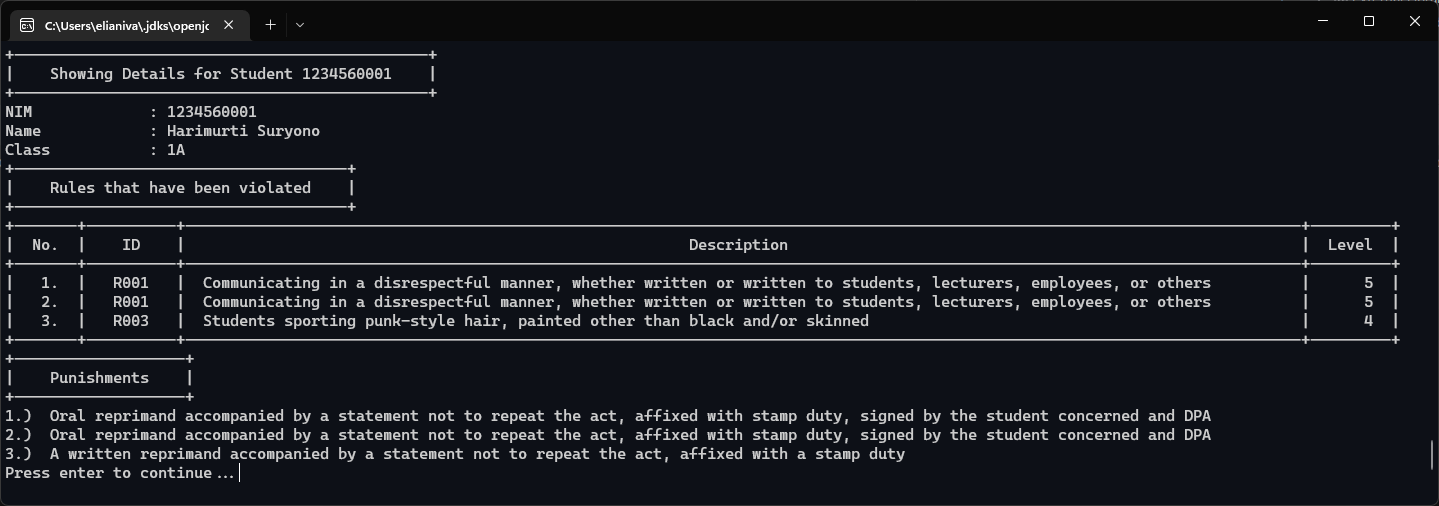
\includegraphics[width=.8\textwidth]{images/show-detail.png}
    \caption{The app showing Student's detail}
\end{figure}

\pagebreak

\subsubsection{Adding a New Student}
To add a new student, pick the \textbf{Add Student} menu. The app should ask for the student details.
After inserting all of the students detail, the app should print a success message.

\begin{figure}[h]
    \centering
    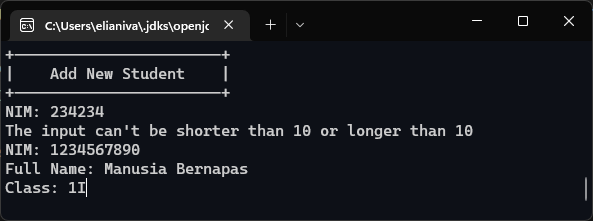
\includegraphics[width=.8\textwidth]{images/add-student-input.png}
    \caption{The app asking for student's data and showing a warning on invalid input}
\end{figure}

If a student with the same NIM already exists, the app will print a warning and ask for a new student's detail.

\begin{figure}[h]
    \centering
    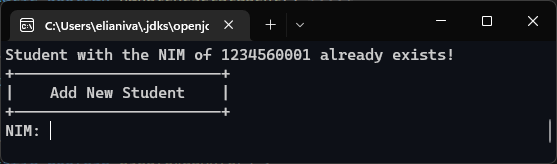
\includegraphics[width=.8\textwidth]{images/add-student-warning.png}
    \caption{The app showing a warning because the student already exists}
\end{figure}

\pagebreak

\subsubsection{Removing a Student}
Removing a student is quite straight forward. Select the \textbf{Remove Student} menu and the app should ask for a NIM.
If the student exists, a success message should be printed. Otherwise, a warning will be printed and
the app will ask for another NIM.

\begin{figure}[h]
    \centering
    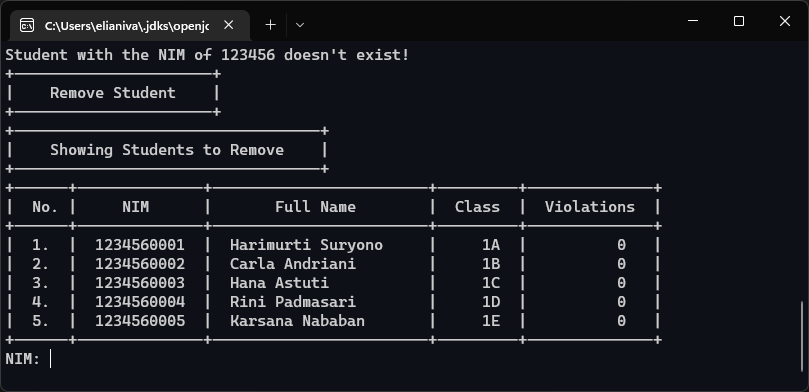
\includegraphics[width=.8\textwidth]{images/remove-student-warning.png}
    \caption{The app showing a warning because the student doesn't exists}
\end{figure}

\begin{figure}[h]
    \centering
    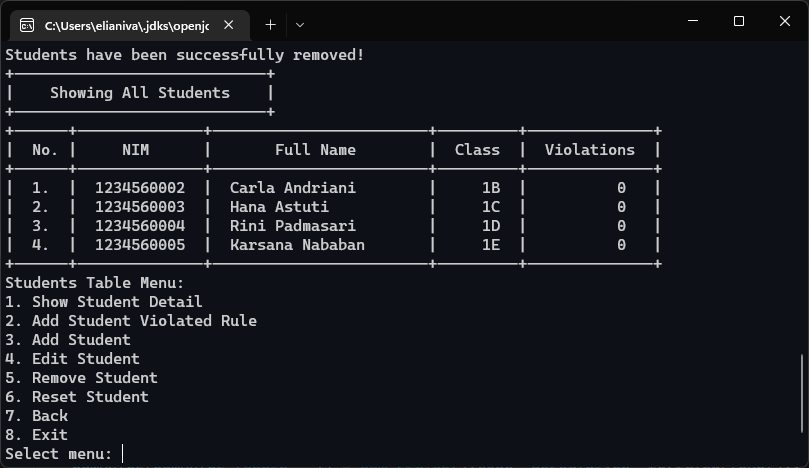
\includegraphics[width=.8\textwidth]{images/remove-student-success.png}
    \caption{The app showing a success message because the student has been deleted}
\end{figure}

\pagebreak

\subsubsection{Editing a Student}
To edit a student's data, pick the TODO menu. The app will ask for a NIM and if the student with that NIM is found,
the app will continue to ask for other details. Otherwise, a warning message saying that the student doesn't exist should be printed.

\begin{figure}[h]
    \centering
    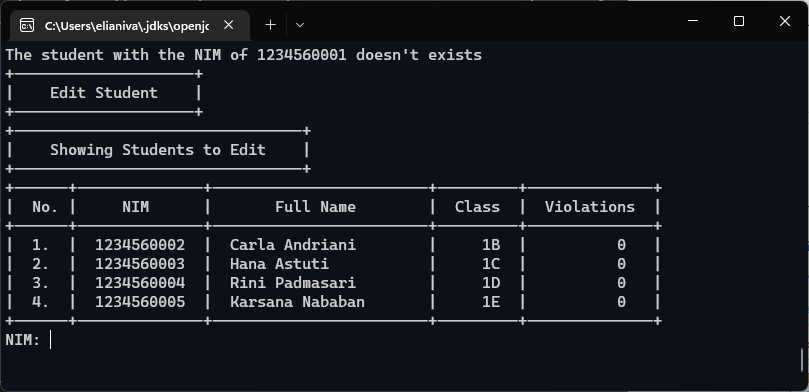
\includegraphics[width=.8\textwidth]{images/edit-student-warning.png}
    \caption{The app showing a warning because the student doesn't exists}
\end{figure}

To preserve the old data, simply leave the input empty like shown below:

\begin{figure}[h]
    \centering
    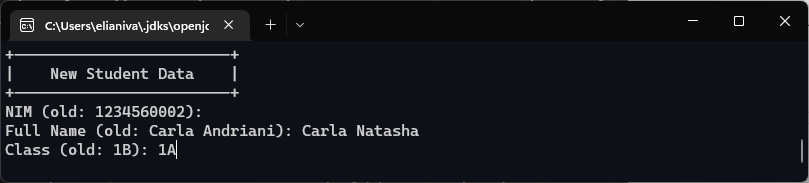
\includegraphics[width=.8\textwidth]{images/edit-student-input.png}
    \caption{The app asking for the new studen'ts detail}
\end{figure}

\pagebreak

After inserting the new Student data, the app will check if the new NIM will conflict with the old one.
If it doesn't then the app will modify the old data with the new one, otherwise a print warning will be printed
and the app will ask again for the new student data.

\begin{figure}[h]
    \centering
    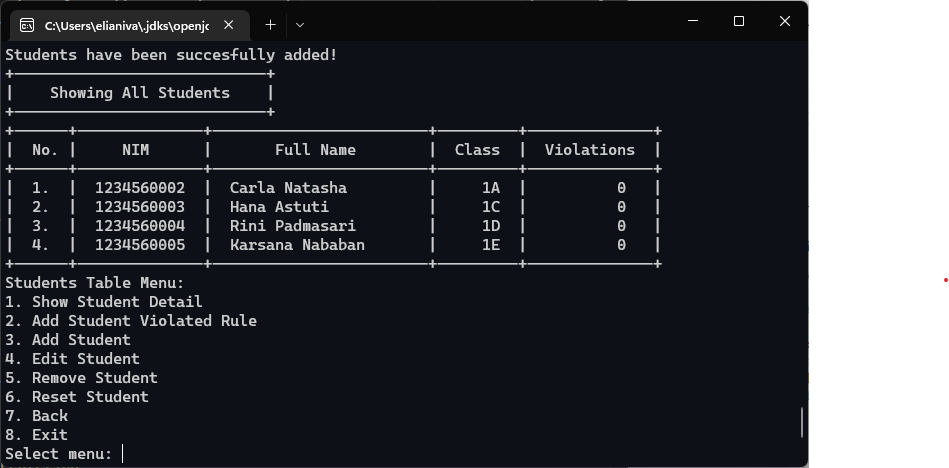
\includegraphics[width=.8\textwidth]{images/edit-student-success.png}
    \caption{The app showing a success message because the student has been edited}
\end{figure}

\subsubsection{Reset a Student}
When a student has maxed out their limit, a reset needs to be done before adding a new violated rule.
To perform this, select the \textbf{Reset Student} menu and the app should ask for a student's NIM.

\begin{figure}[h]
    \centering
    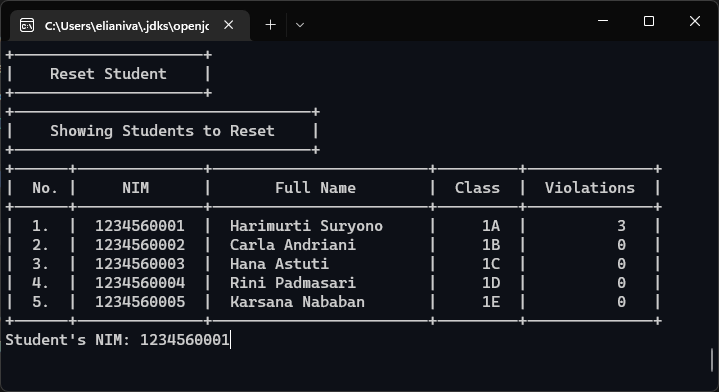
\includegraphics[width=.8\textwidth]{images/reset-student-input.png}
    \caption{The app asking a student's NIM to reset}
\end{figure}

\pagebreak

When the NIM is valid, the app should display a success message

\begin{figure}[h]
    \centering
    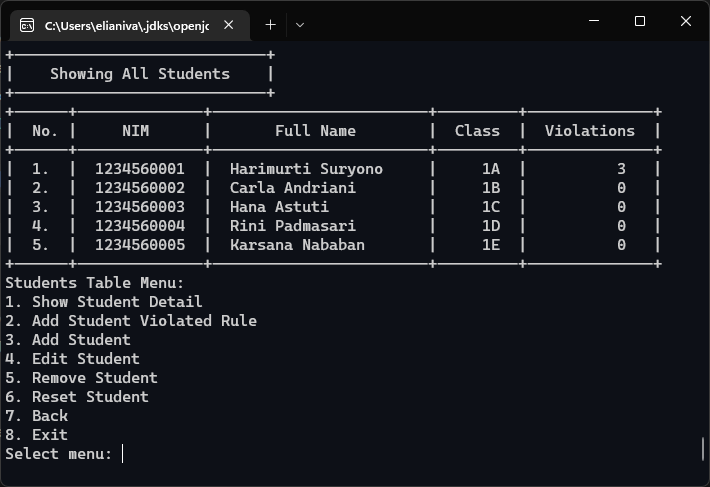
\includegraphics[width=.8\textwidth]{images/reset-student-success.png}
    \caption{The app showing a success message after resetting a student}
\end{figure}

\pagebreak

\subsection{Rules Menu}
On the main menu, choose the second menu to show a list of actions related to Rules operations.
The app should now display all rules along with their menu.

\begin{figure}[h]
    \centering
    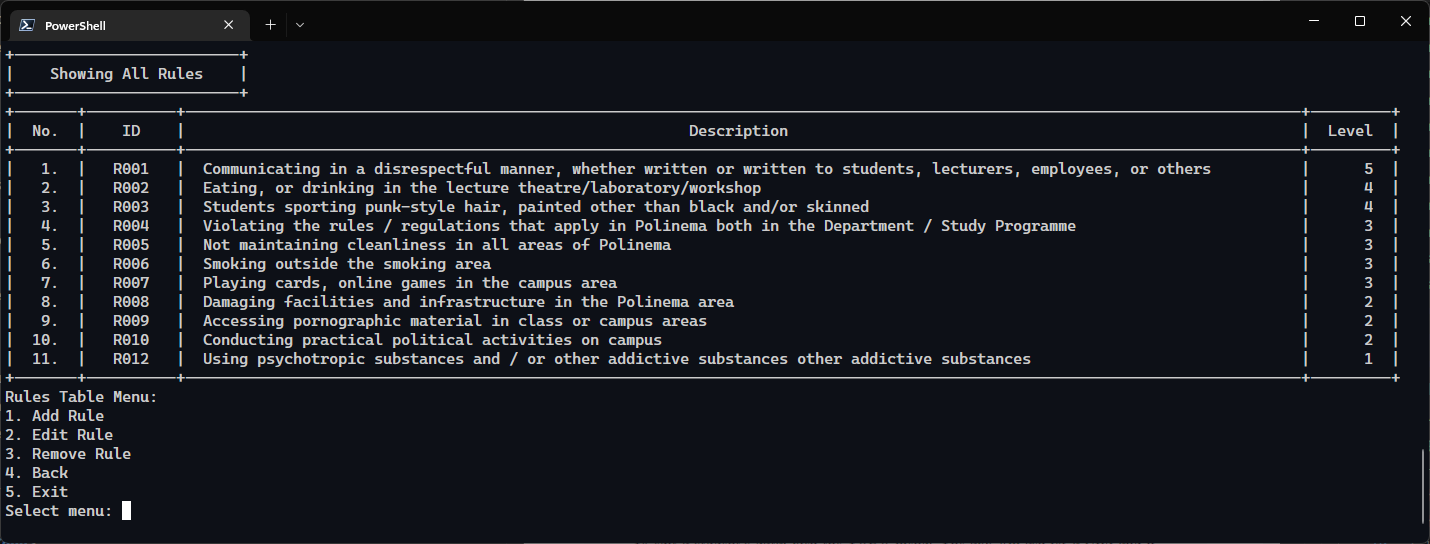
\includegraphics[width=\textwidth]{images/rule-menu.png}
    \caption{The app showing rules list along with their menu}
\end{figure}

\subsubsection{Rule Entity}
Before going with the rest of the menu, there are some things that should be noted.
These are some details regarding each Student entity along with its validation

\begin{enumerate}
    \item {
        \textbf{Code}
        \begin{itemize}
            \item Min Length: 4 characters
            \item Max Length: 4 characters
            \item Allowed to be empty: No
        \end{itemize}
    }
    \item {
        \textbf{Description}
        \begin{itemize}
            \item Min Length: 10 character
            \item Max Length: 120 characters
            \item Allowed to be empty: No
        \end{itemize}
    }
    \item {
        \textbf{Level}
        \begin{itemize}
            \item Min: 1
            \item Max: 5
            \item Allowed to be empty: No
        \end{itemize}
    }
\end{enumerate}

\pagebreak

\subsubsection{Adding a New Rule}
To add a new rule, pick the \textbf{Add Rule} menu. The app should ask for the rule details.
After inserting all of the rule details, the app should print a success message.

\begin{figure}[h]
    \centering
    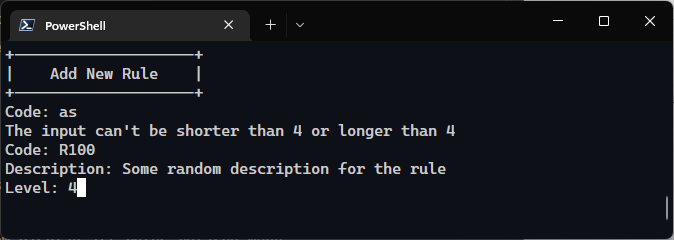
\includegraphics[width=.8\textwidth]{images/add-rule-input.png}
    \caption{The app asking for rule's data and showing a warning on invalid input}
\end{figure}

If a rule with the same code already exists, the app will print a warning and ask for a new rule detail.

\begin{figure}[h]
    \centering
    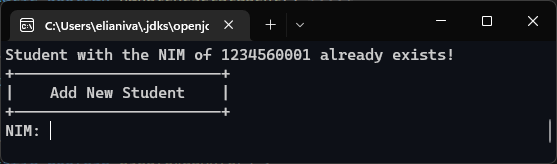
\includegraphics[width=.8\textwidth]{images/add-student-warning.png}
    \caption{The app asking for rule's data and showing a warning on invalid input}
\end{figure}

\pagebreak

\subsubsection{Removing a Rule}
Removing a student is quite straight forward. Select the TODO menu and the app should ask for a NIM.
If the student exists, a success message should be printed. Otherwise, a warning will be printed and
the app will ask for another NIM.

\begin{figure}[h]
    \centering
    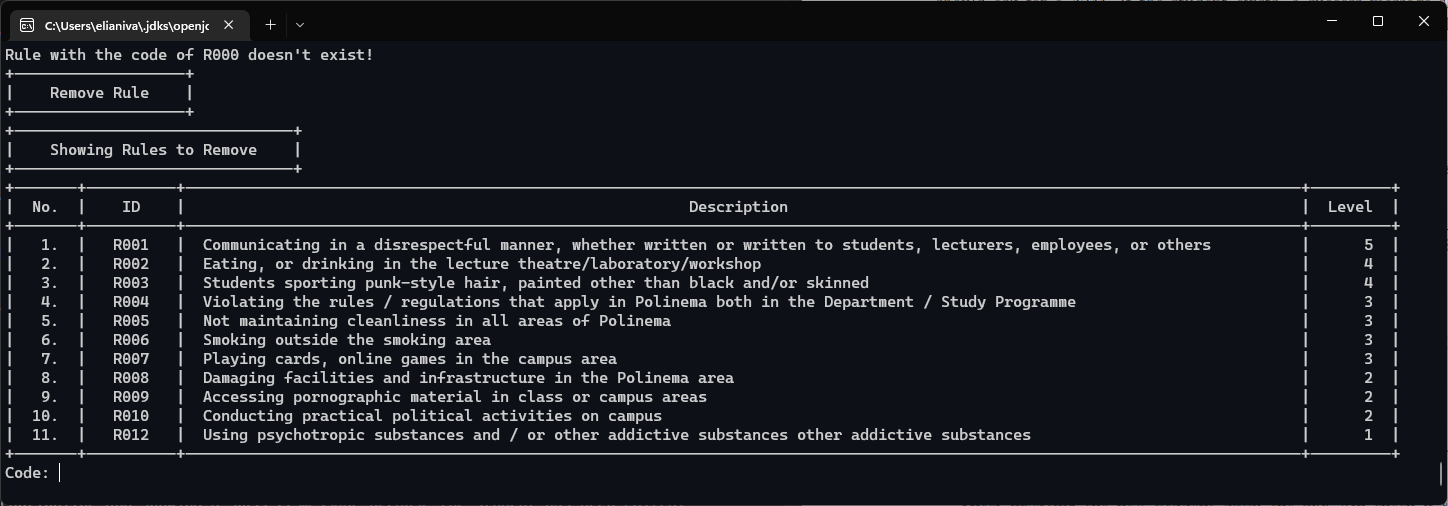
\includegraphics[width=.8\textwidth]{images/remove-rule-warning.png}
    \caption{The app showing a warning because the rule doesn't exist}
\end{figure}

\begin{figure}[h]
    \centering
    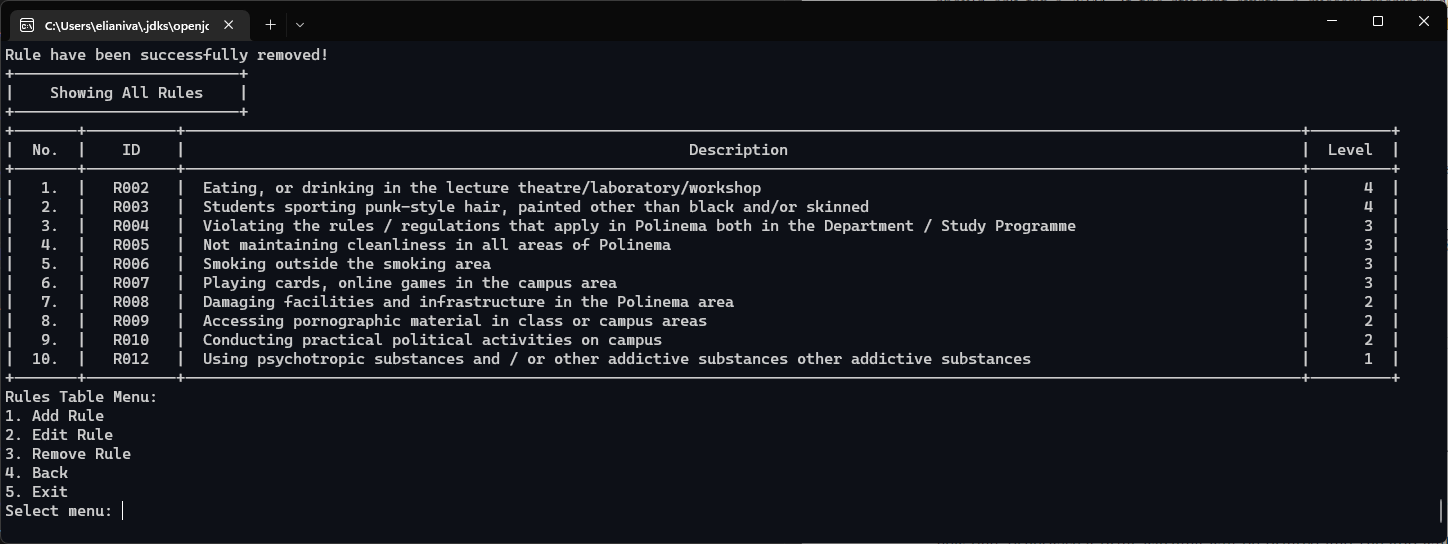
\includegraphics[width=.8\textwidth]{images/remove-rule-success.png}
    \caption{The app showing a success message because the rule has been deleted}
\end{figure}

\pagebreak

\subsubsection{Editing a Rule}
To edit a student's data, pick the TODO menu. The app will ask for a NIM and if the student with that NIM is found,
the app will continue to ask for other details. Otherwise, a warning message saying that the student doesn't exist should be printed.

\begin{figure}[h]
    \centering
    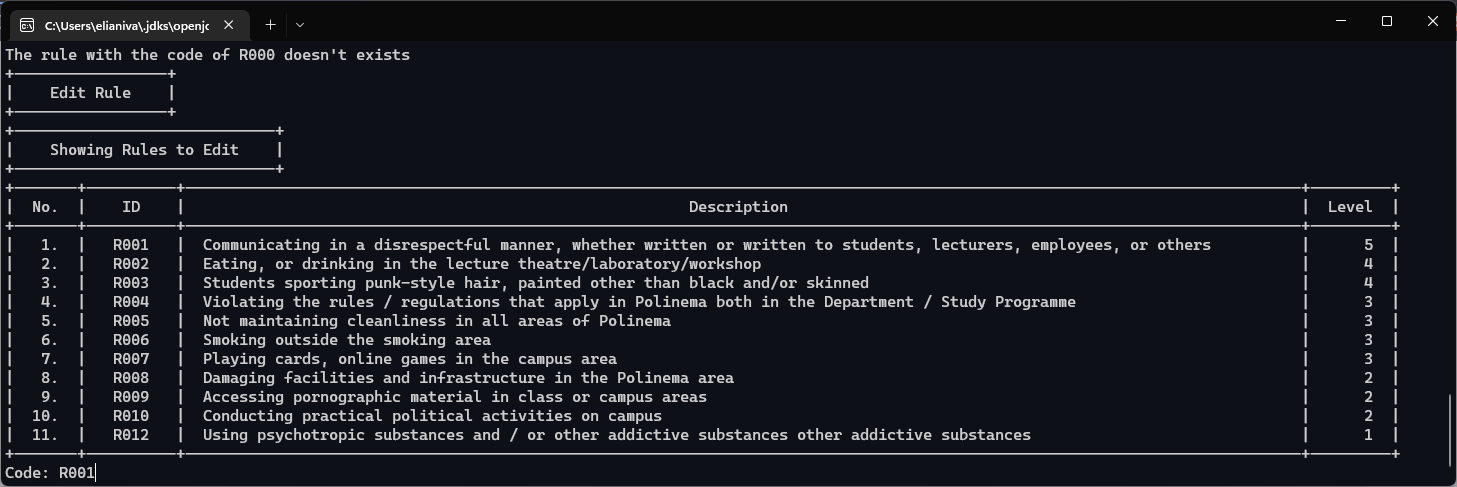
\includegraphics[width=.8\textwidth]{images/edit-rule-input.png}
    \caption{The app asking for a rule id and warning}
\end{figure}

After inserting the new Student data, the app will check if the new NIM will conflict with the old one.
If it doesn't then the app will modify the old data with the new one, otherwise a print warning will be printed
and the app will ask again for the new student data.

\begin{figure}[h]
    \centering
    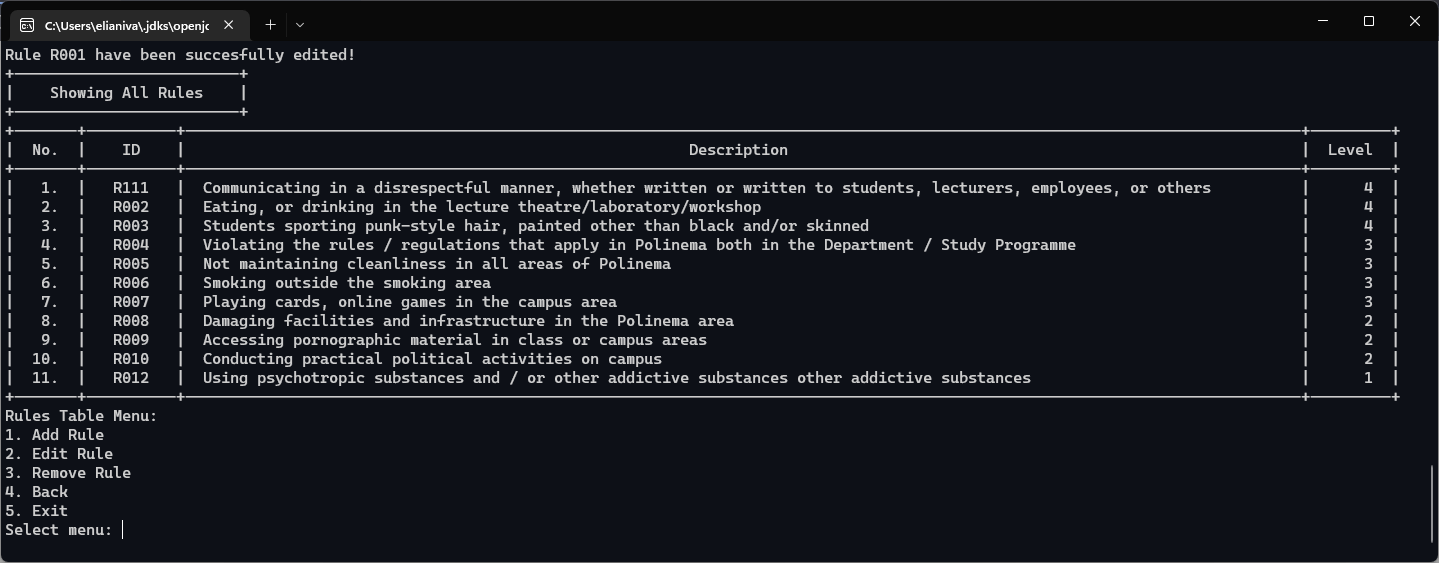
\includegraphics[width=.8\textwidth]{images/edit-rule-success.png}
    \caption{The app showing a success message}
\end{figure}

\pagebreak

\section{Flowchart}
These section describes the flow of the application using a flowchart. All of these flowcharts are made using
MermaidJS.

\subsection{Main Menu}

\begin{figure}[h]
    \begin{minipage}{.45\textwidth}
        \centering
        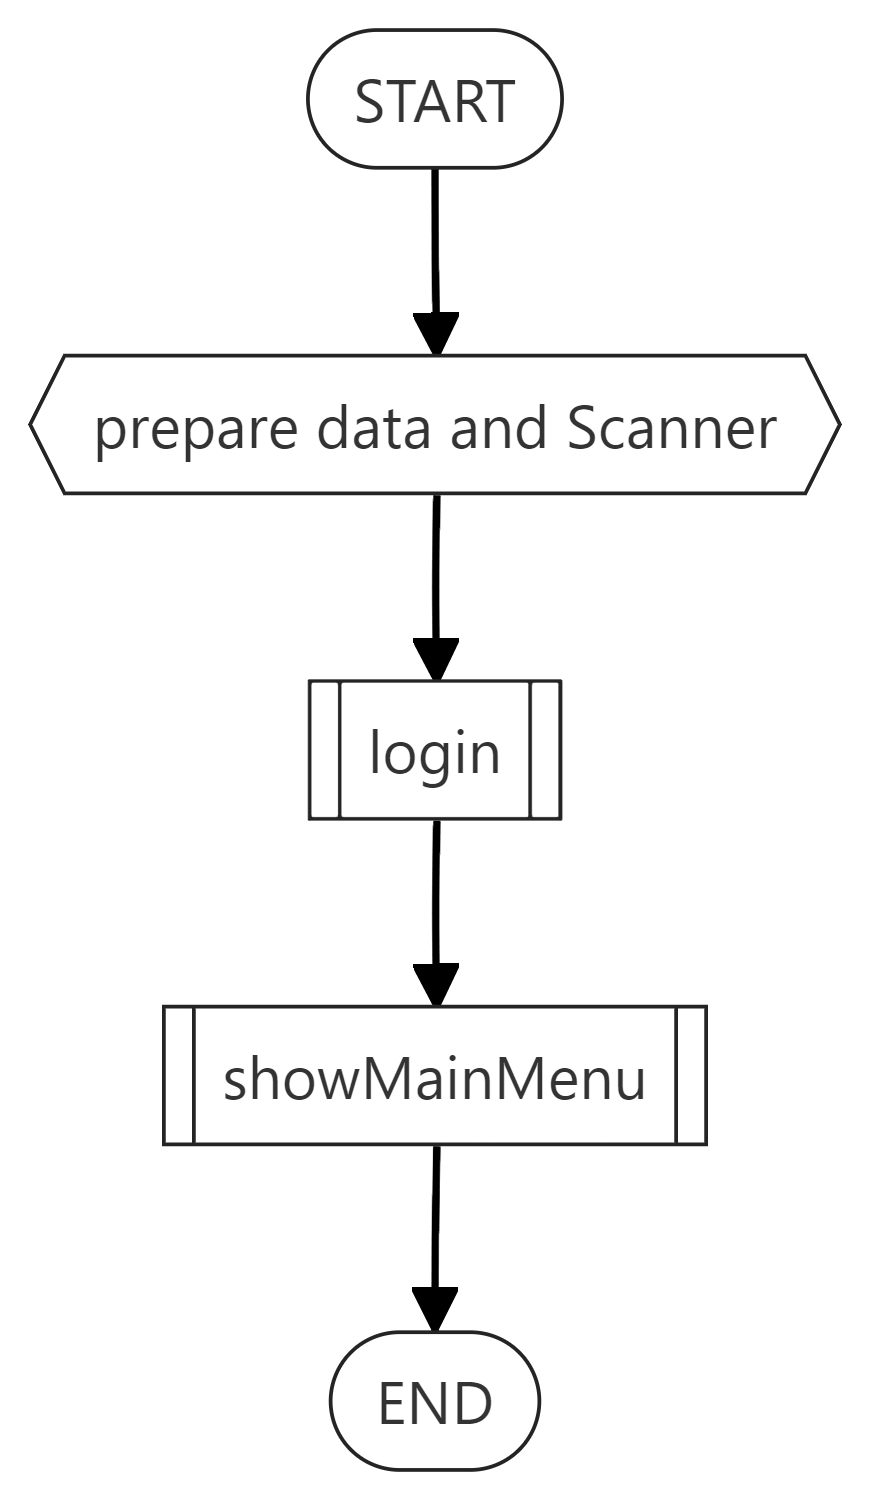
\includegraphics[width=4cm]{flowcharts/main.png}
        \captionof{figure}{\texttt{Main(String[] args)}}
    \end{minipage}
    \begin{minipage}{.5\textwidth}
        \centering
        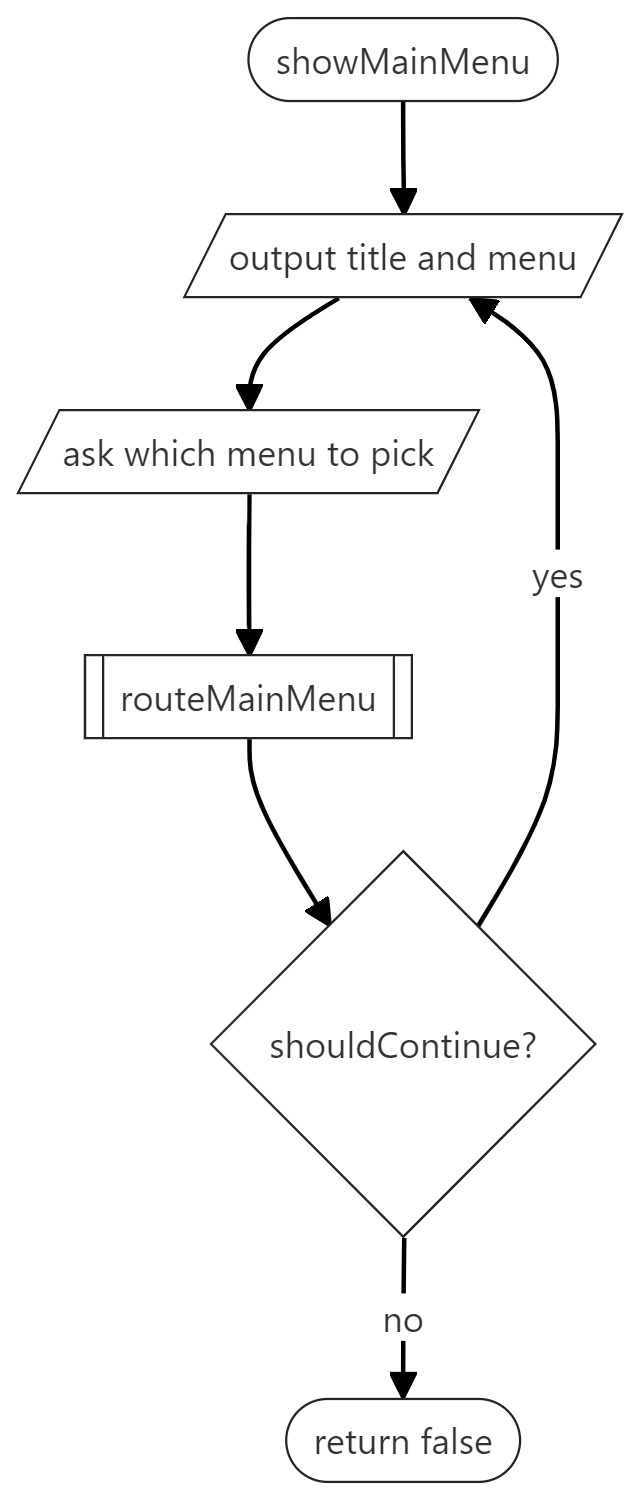
\includegraphics[width=4cm]{flowcharts/main-menu.png}
        \captionof{figure}{\texttt{showMainMenu()}}
    \end{minipage}
\end{figure}

\begin{figure}[h]
    \centering
    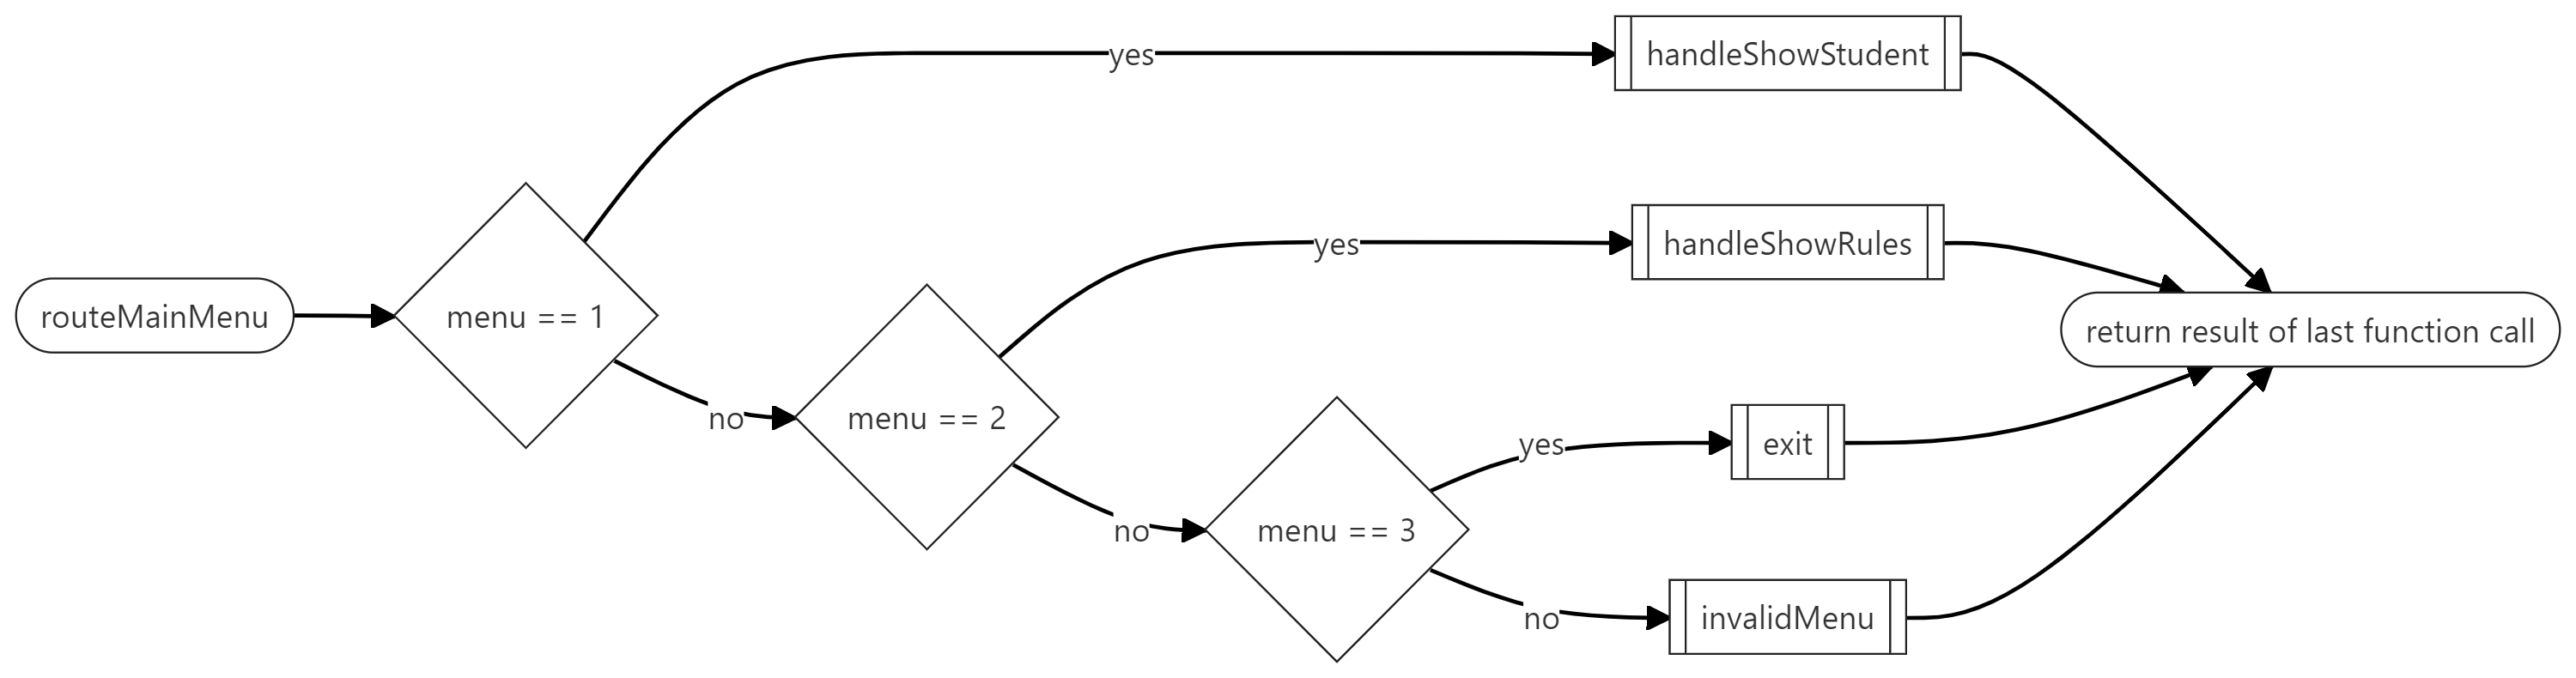
\includegraphics[width=.9\textwidth]{flowcharts/route-main-menu.png}
    \caption{\texttt{routeMainMenu(int chosenMenu)}}
\end{figure}

\pagebreak

\begin{figure}[h]
    \centering
    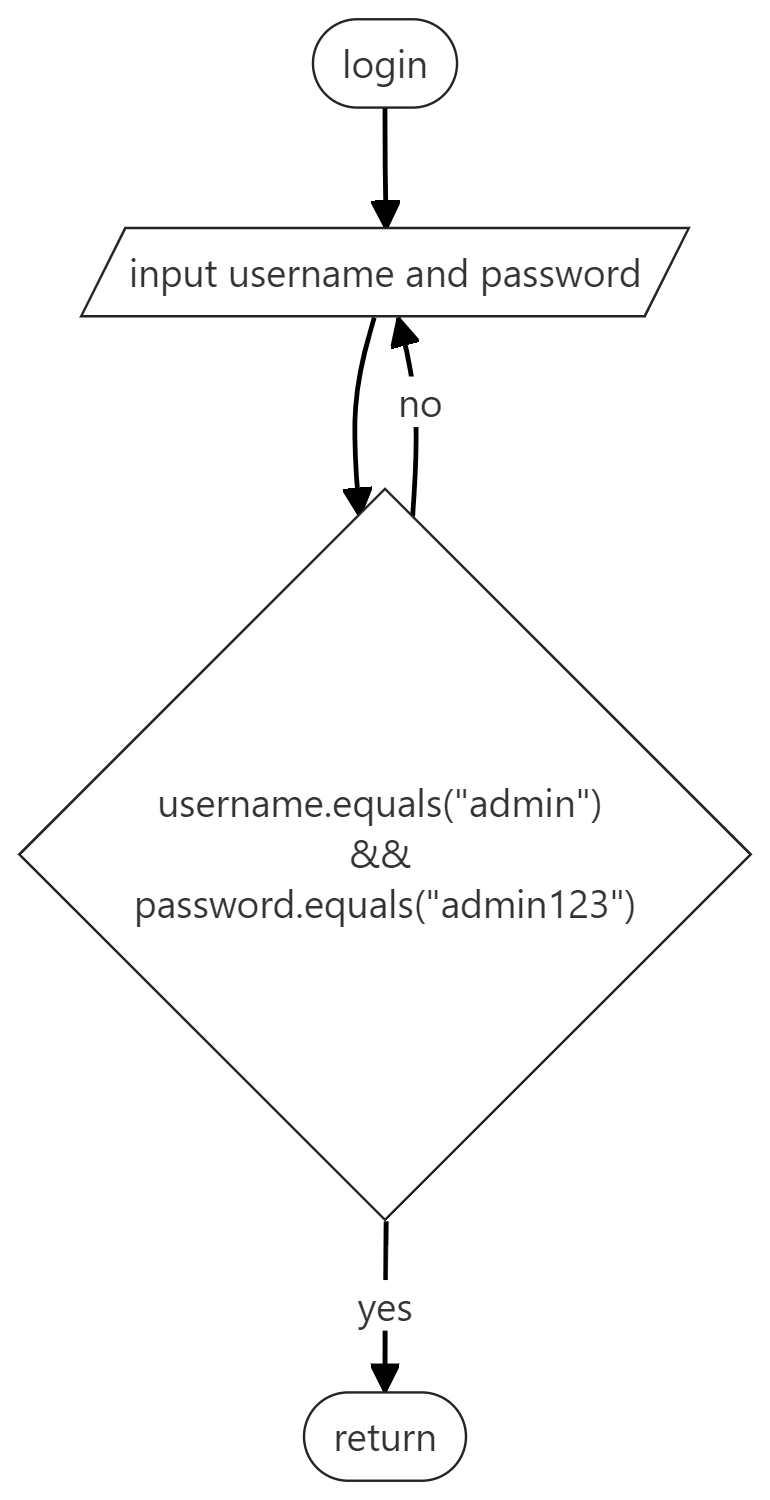
\includegraphics[width=8cm]{flowcharts/login.png}
    \caption{\texttt{login()}}
\end{figure}

\pagebreak

\subsection{Students Menu}

\begin{figure}[h]
    \centering
    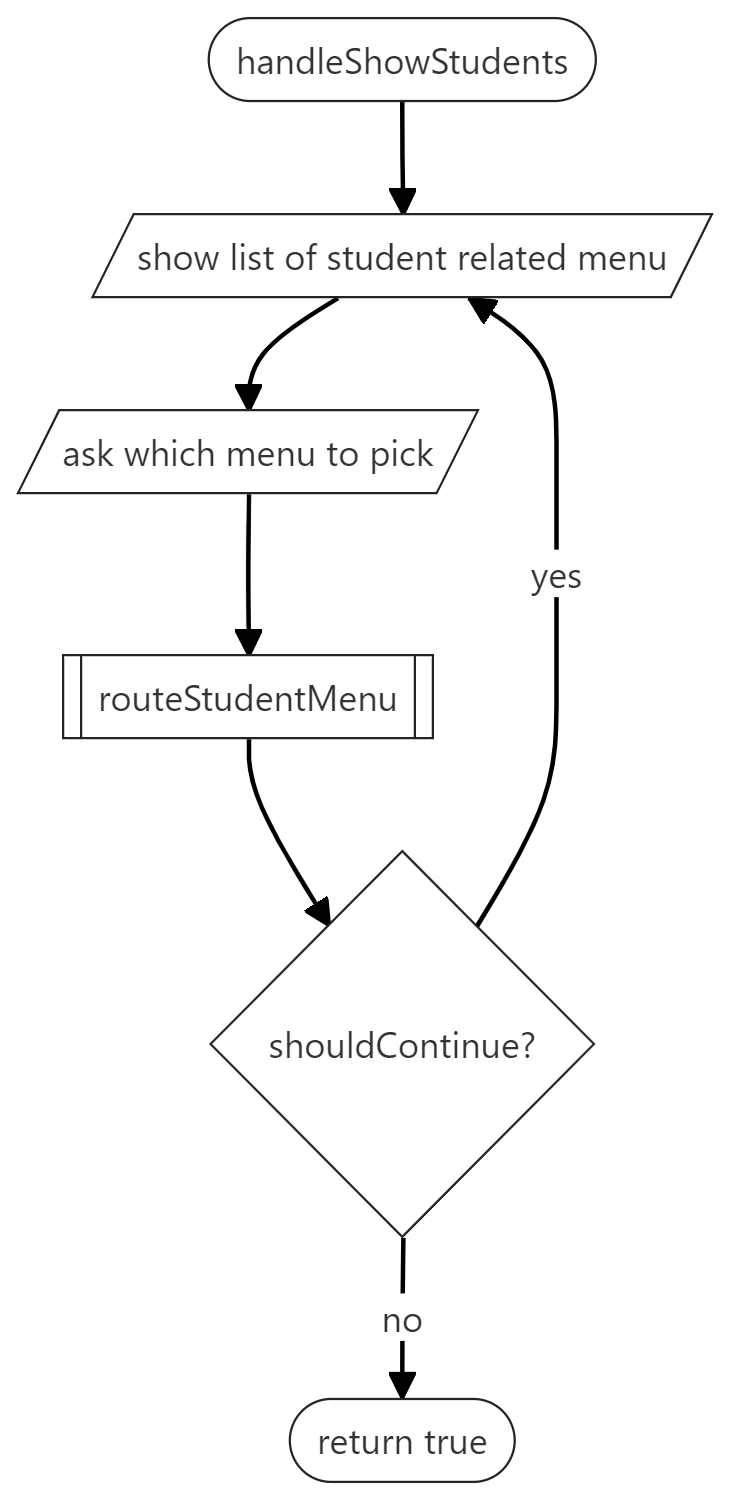
\includegraphics[width=8cm]{flowcharts/student-menu.png}
    \caption{\texttt{handleShowStudents()}}
\end{figure}

\pagebreak

\begin{figure}[h]
    \centering
    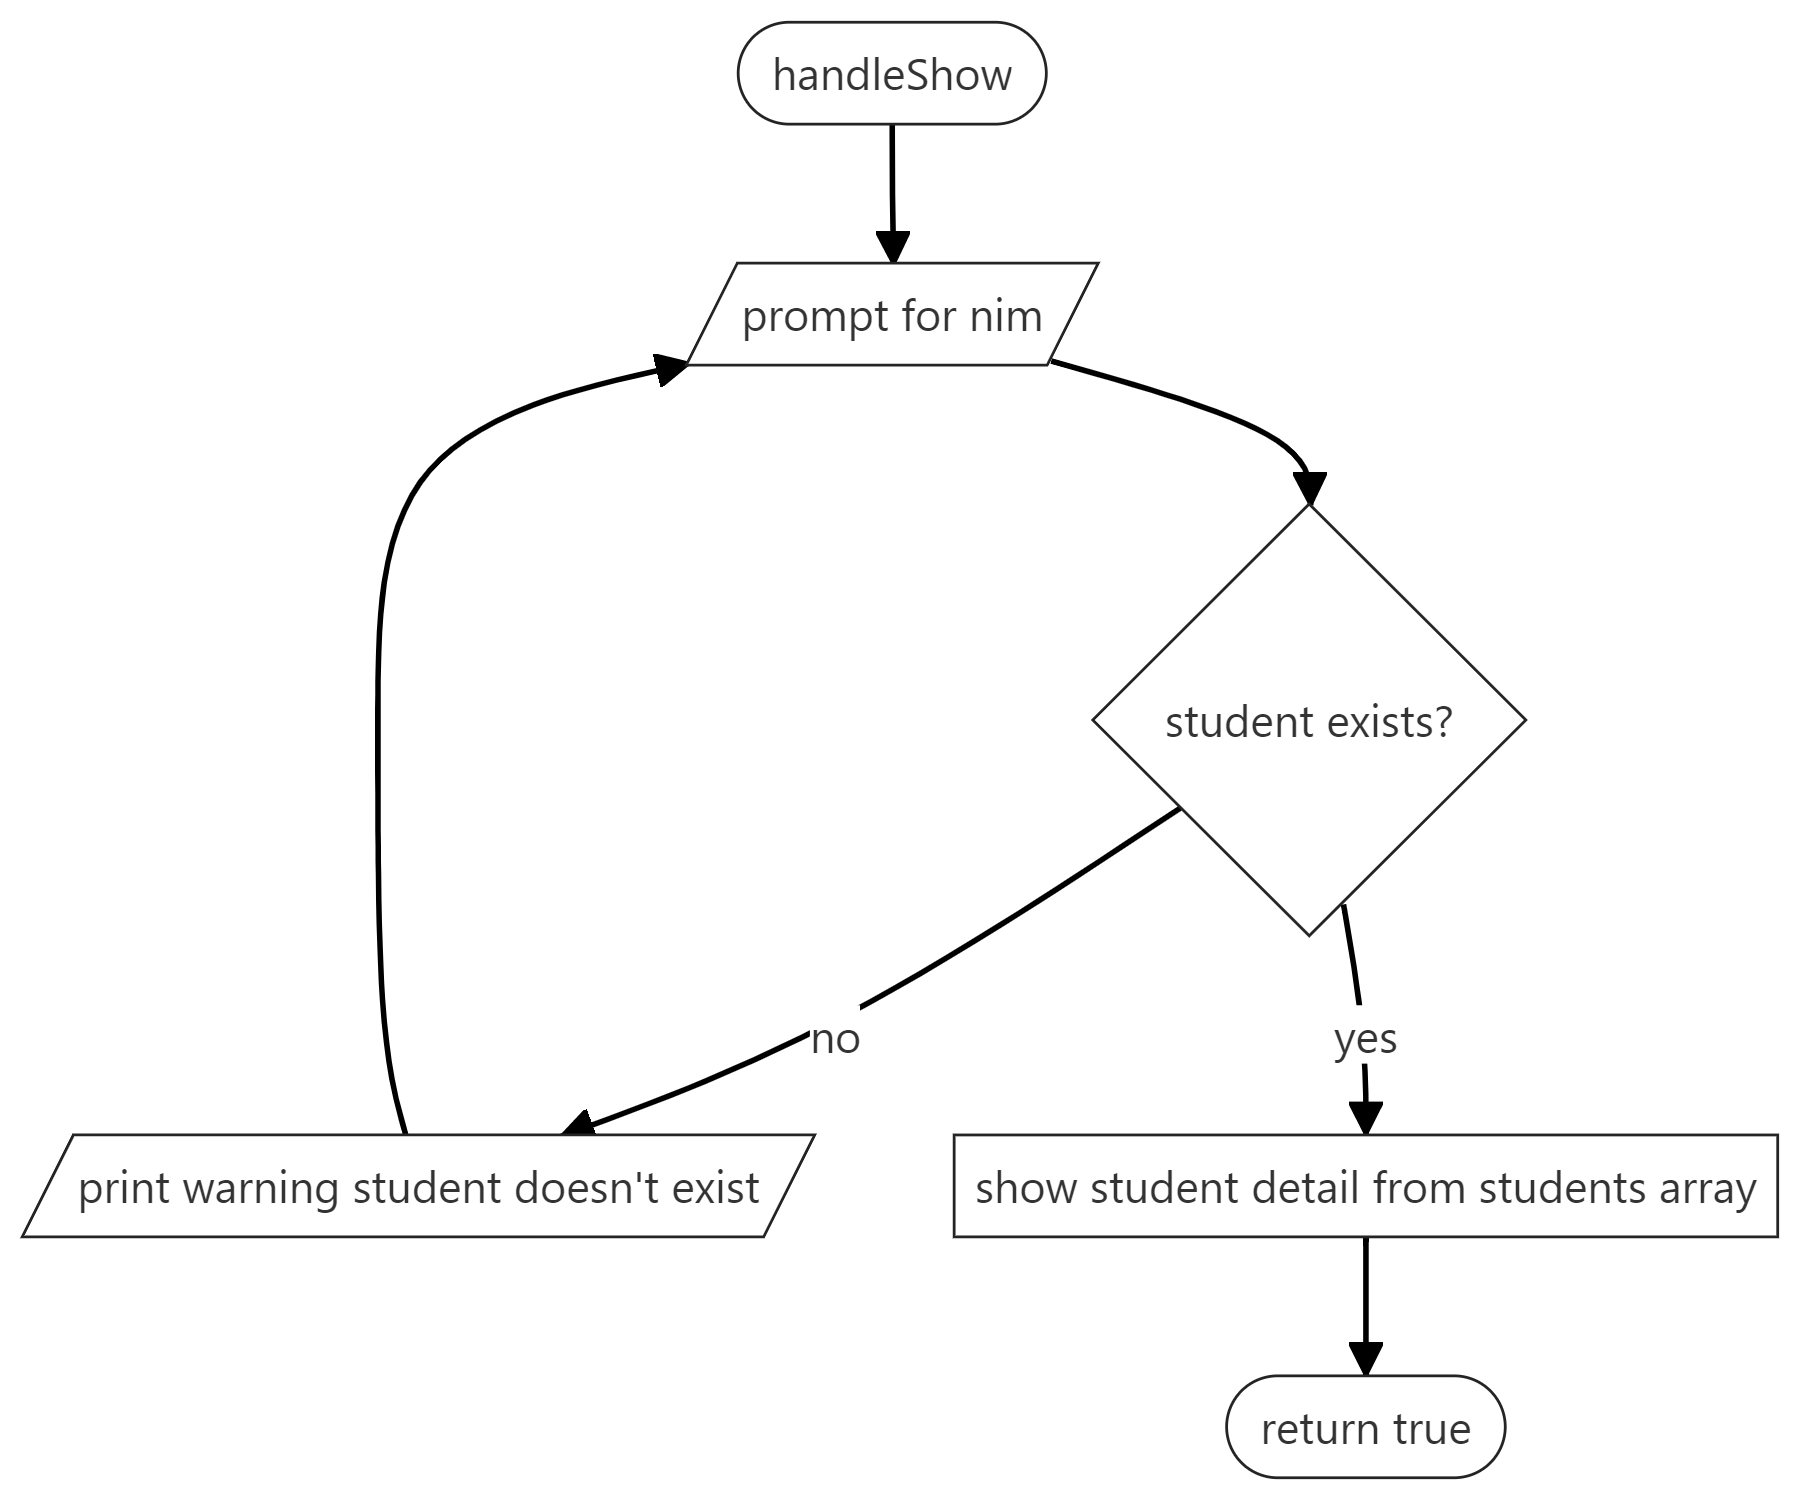
\includegraphics[width=.8\textwidth]{flowcharts/handle-show-student-detail.png}
    \caption{\texttt{handleShowStudentDetail()}}
\end{figure}

\pagebreak

\begin{figure}[h]
    \centering
    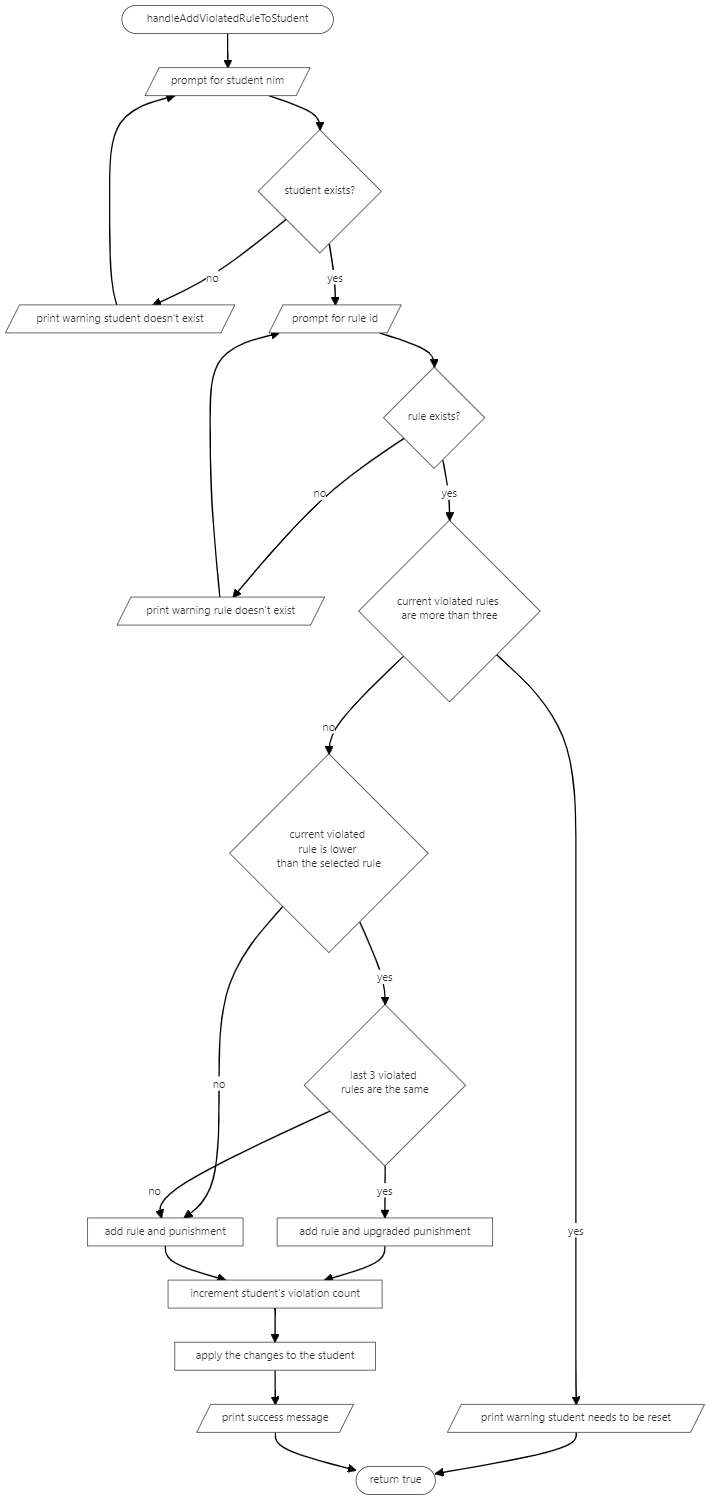
\includegraphics[height=16.75cm]{flowcharts/handle-add-rule-to-student.png}
    \caption{\texttt{handleAddViolatedRuleToStudent()}}
\end{figure}

\pagebreak

\begin{figure}[h]
    \centering
    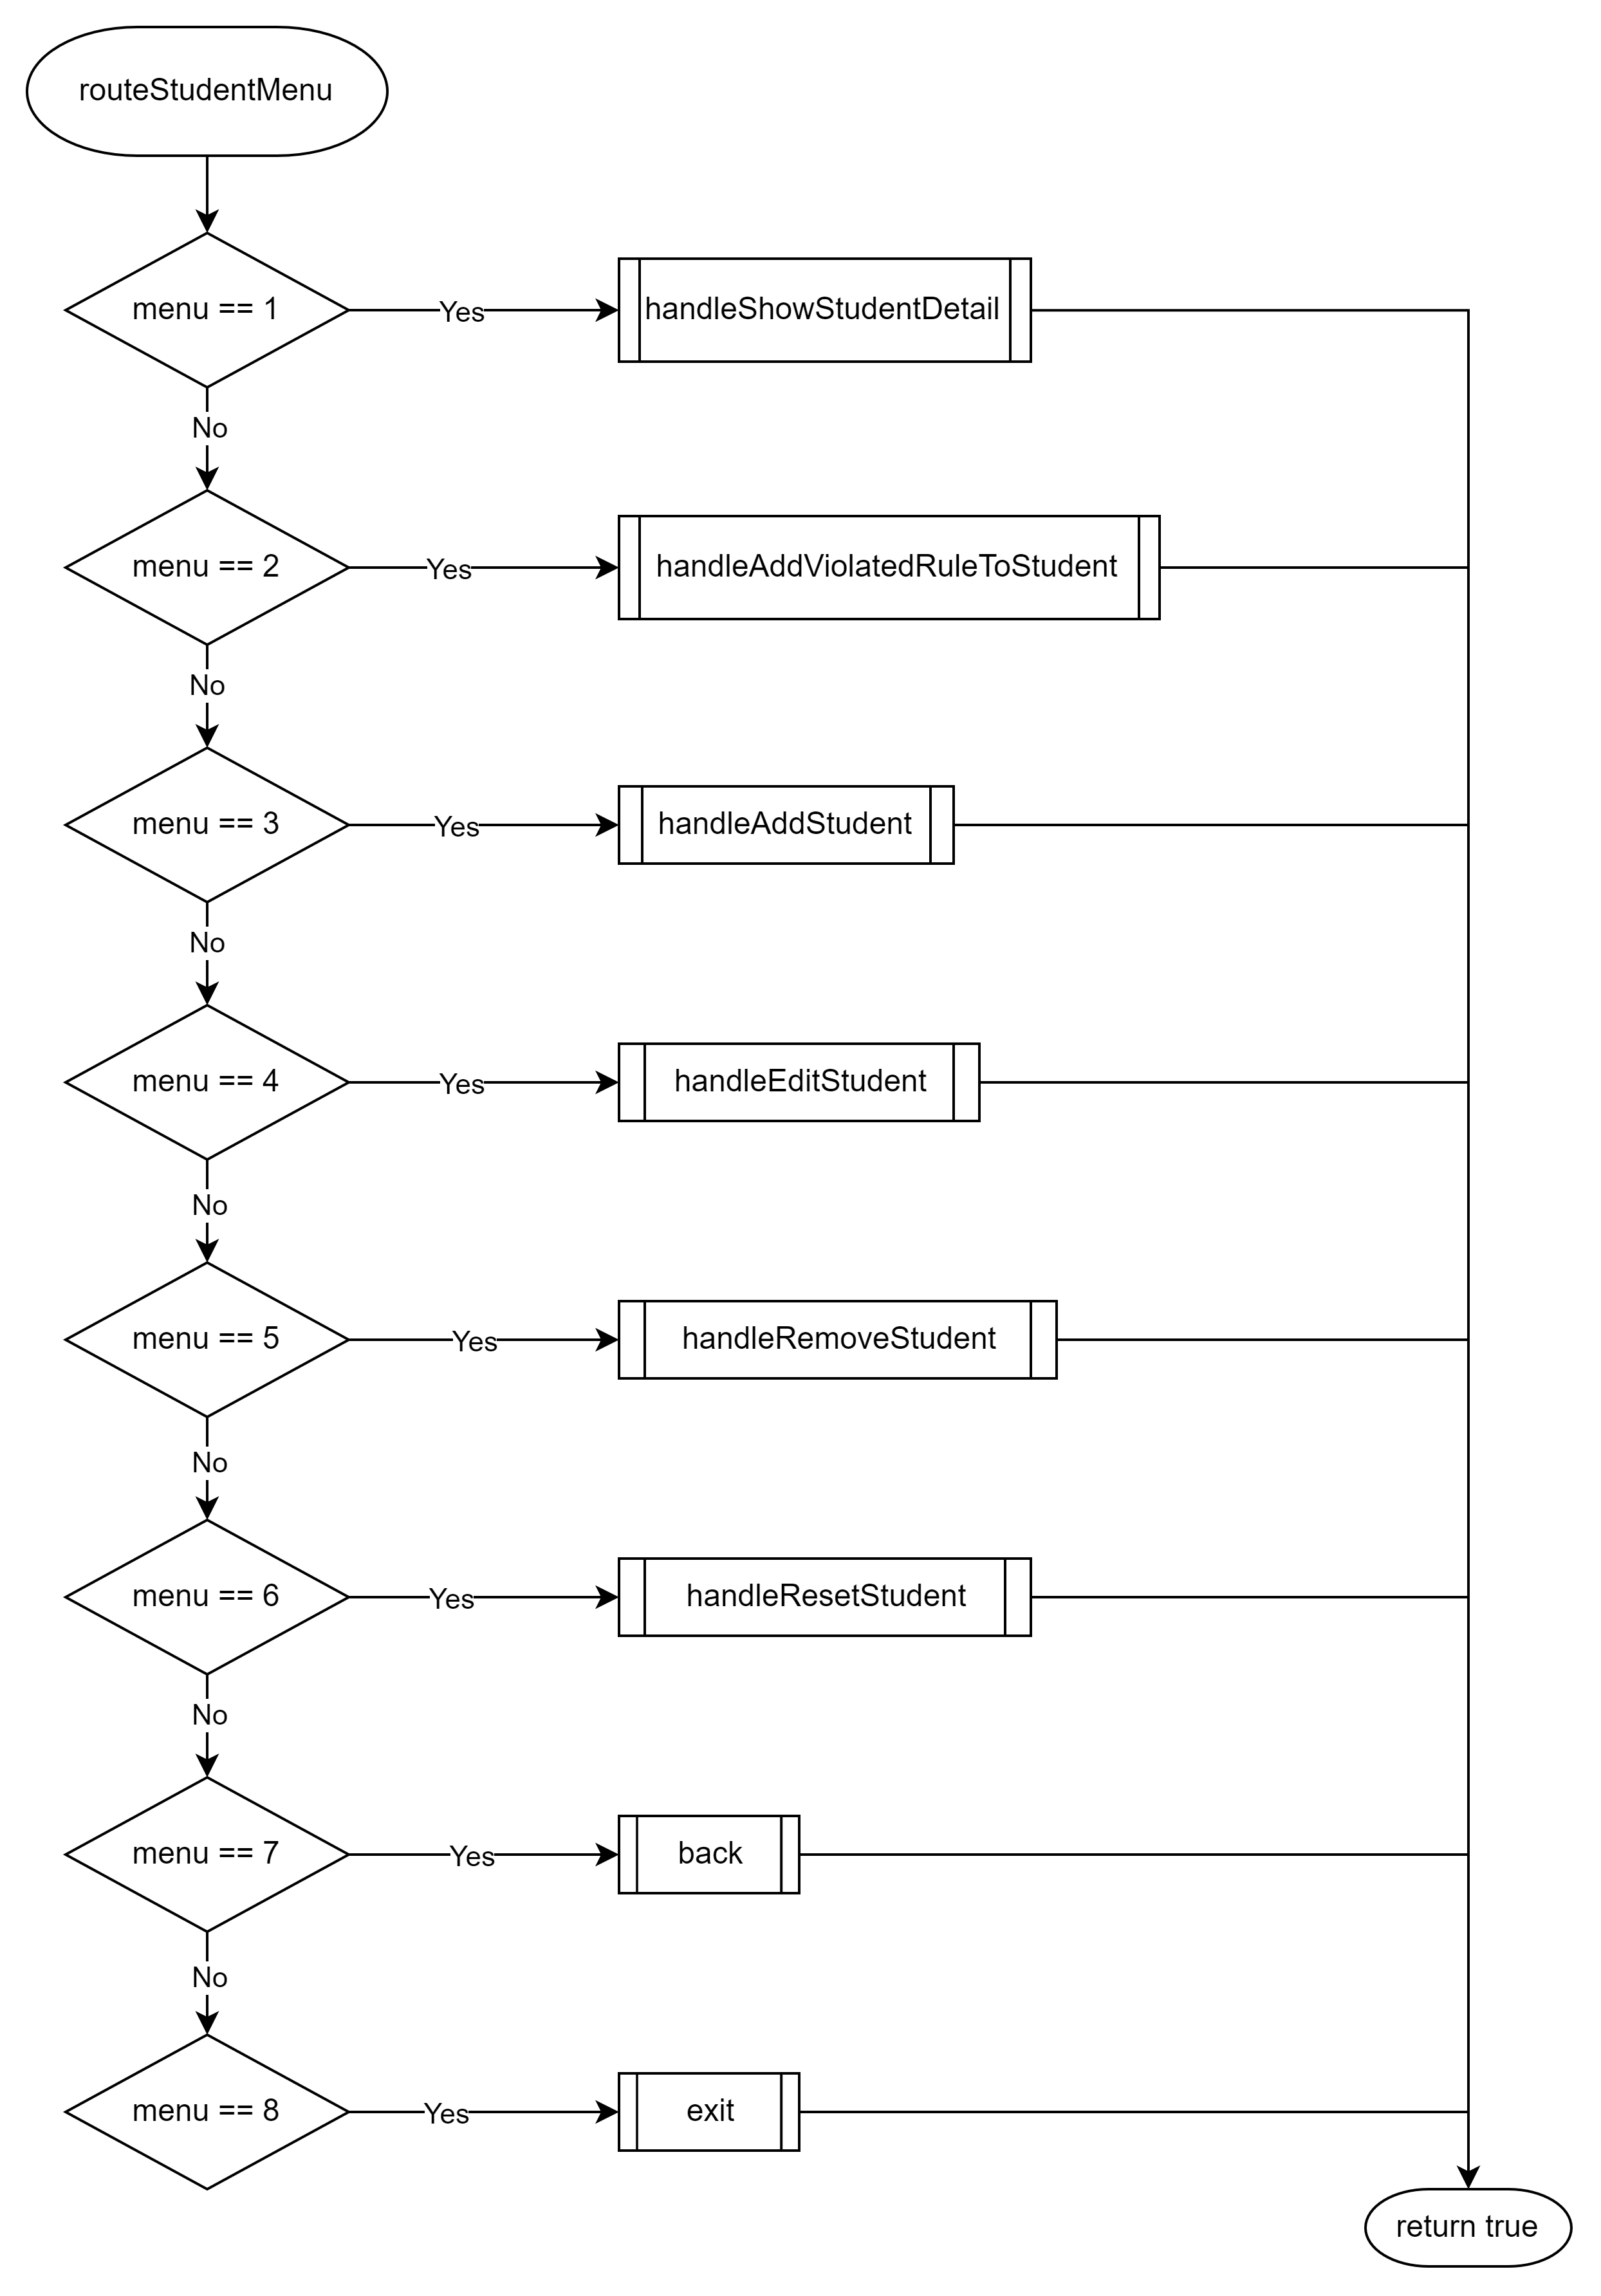
\includegraphics[width=.7\textwidth]{flowcharts/route-student-menu-drawio.png}
    \caption{\texttt{routeStudentMenu(int chosenMenu)}}
\end{figure}

\pagebreak

\begin{figure}[h]
    \centering
    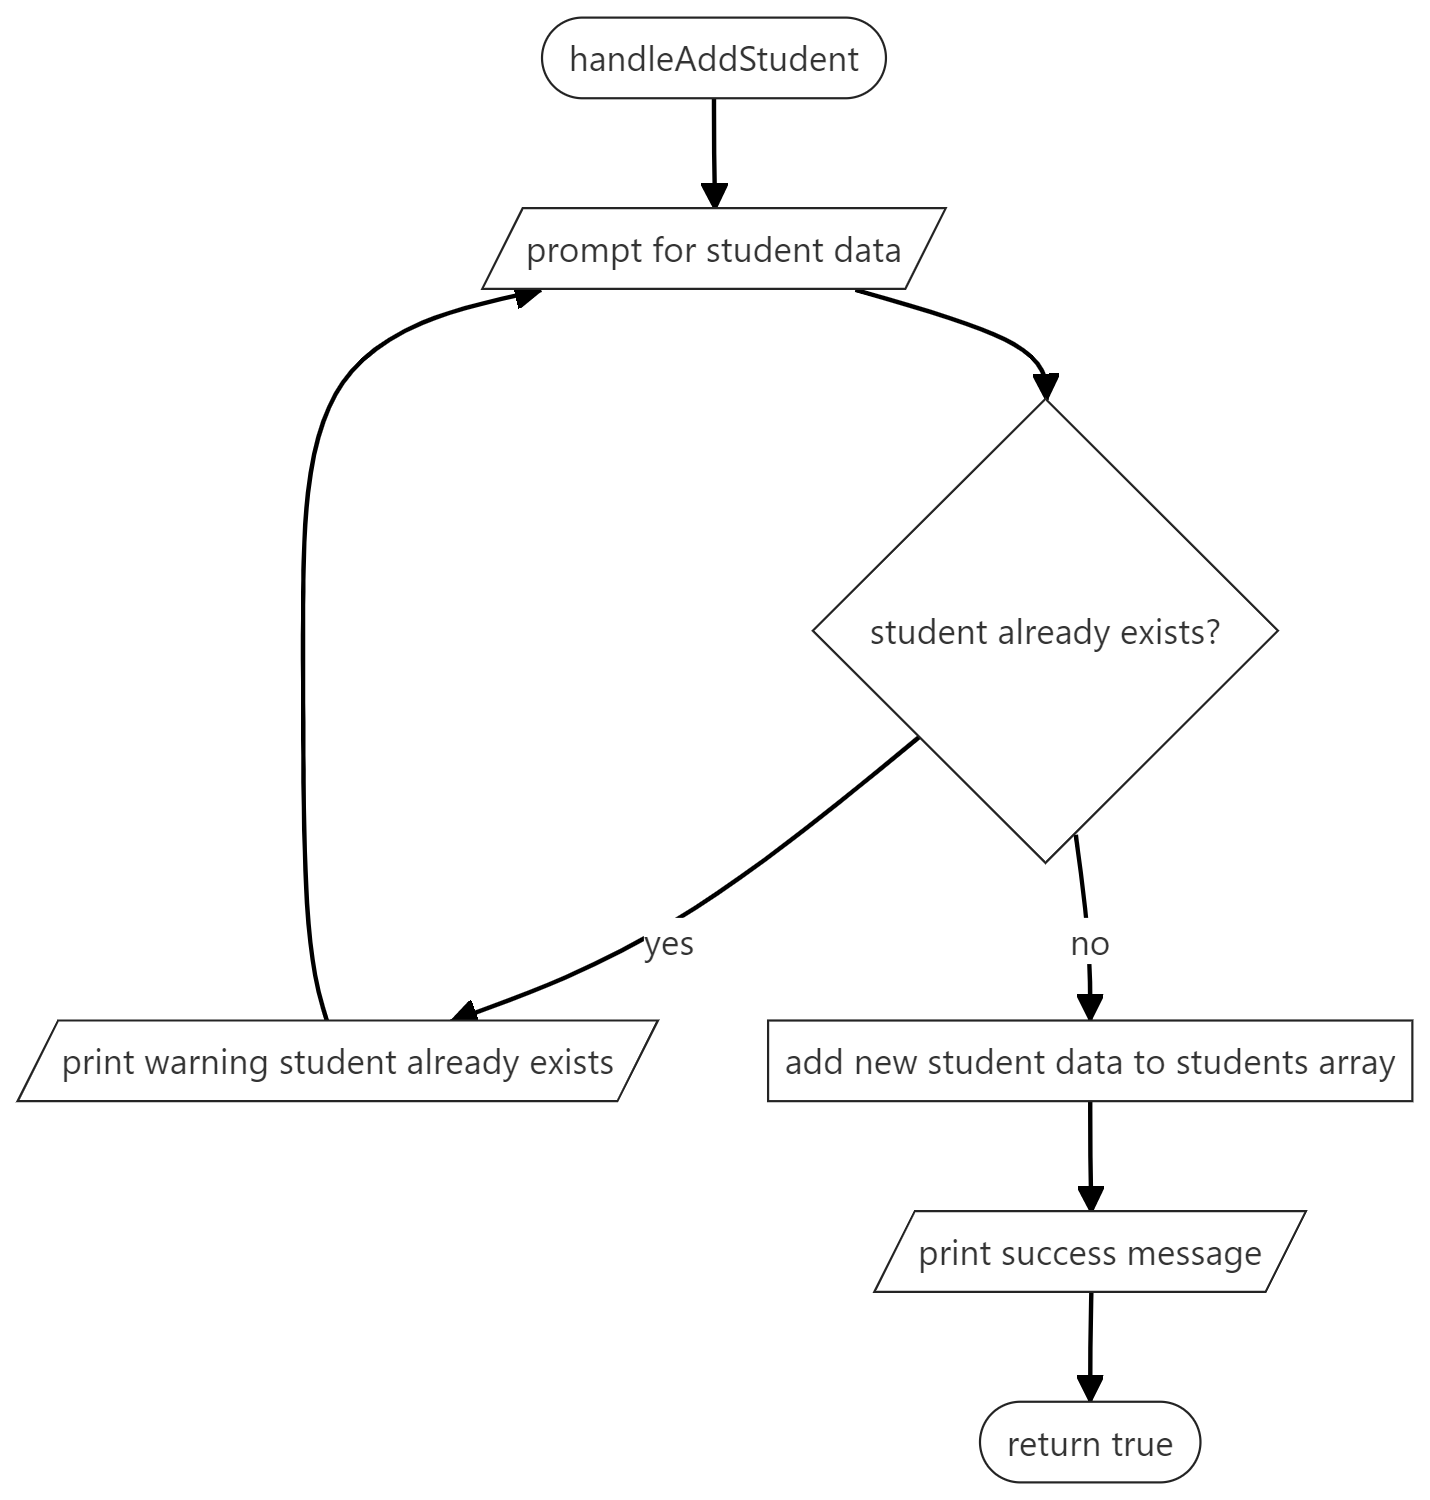
\includegraphics[width=7.2cm]{flowcharts/handle-add-student.png}
    \caption{\texttt{handleAddStudent()}}
\end{figure}

\begin{figure}[h]
    \centering
    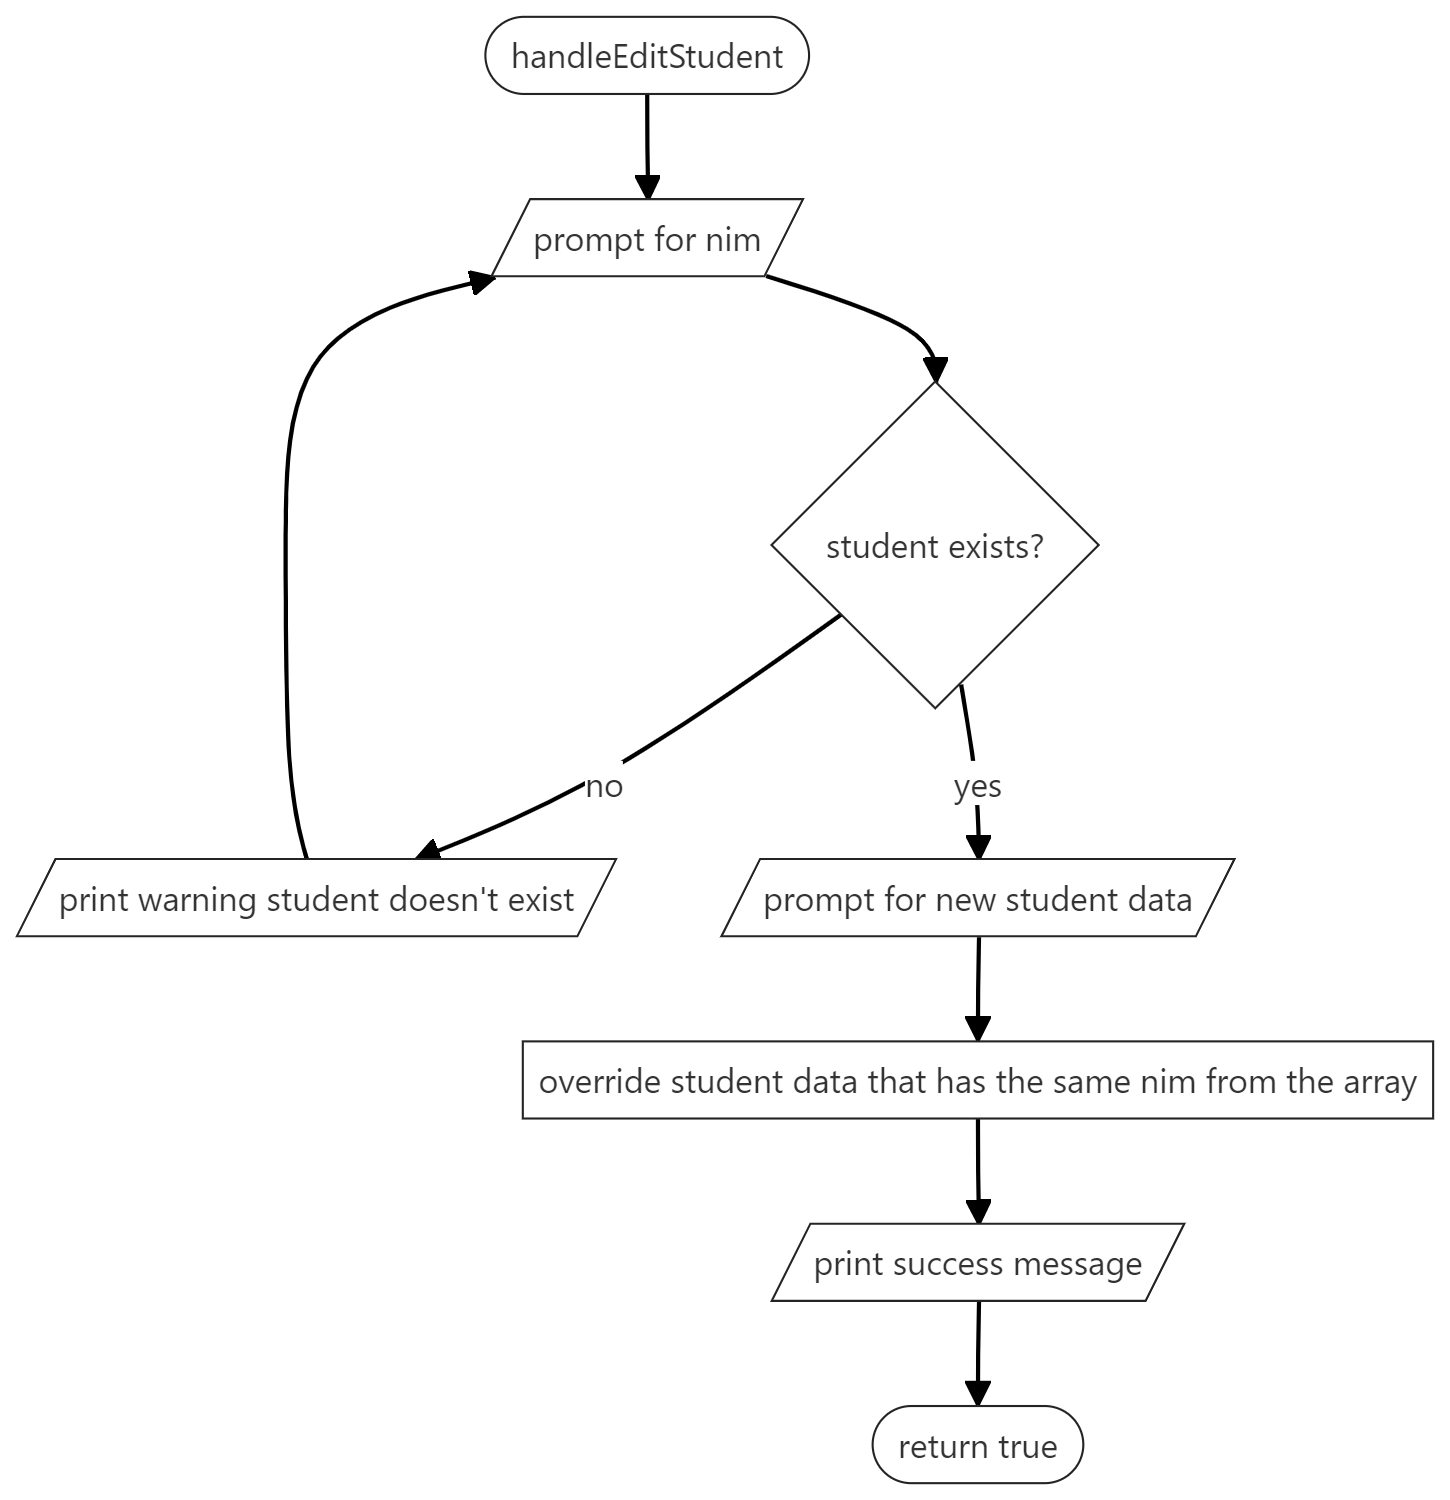
\includegraphics[width=7.2cm]{flowcharts/handle-edit-student.png}
    \caption{\texttt{handleEditStudent()}}
\end{figure}

\pagebreak

\begin{figure}[h]
    \centering
    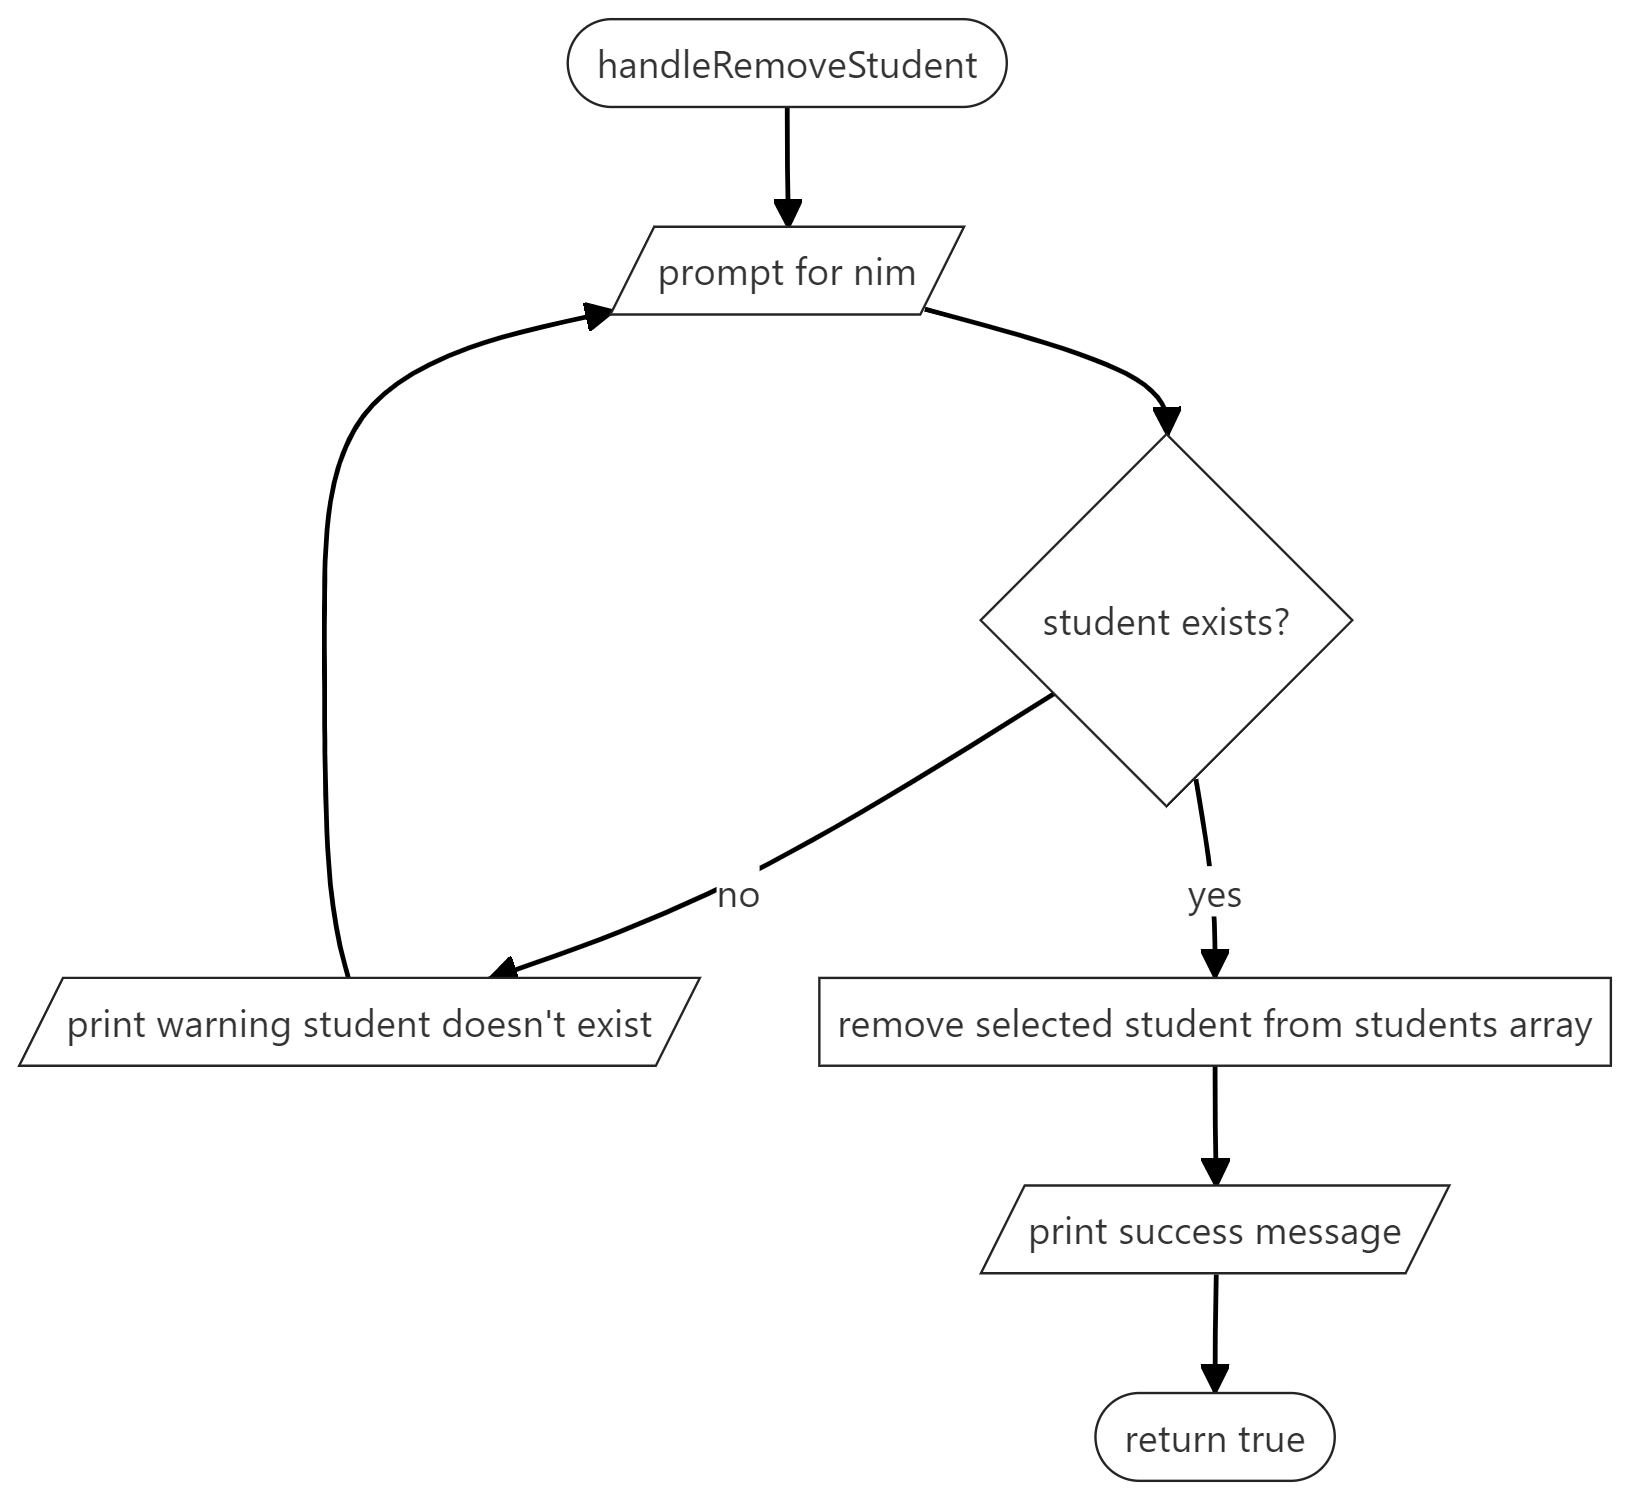
\includegraphics[width=8cm]{flowcharts/handle-remove-student.png}
    \caption{\texttt{handleRemoveStudent()}}
\end{figure}

\begin{figure}[h]
    \centering
    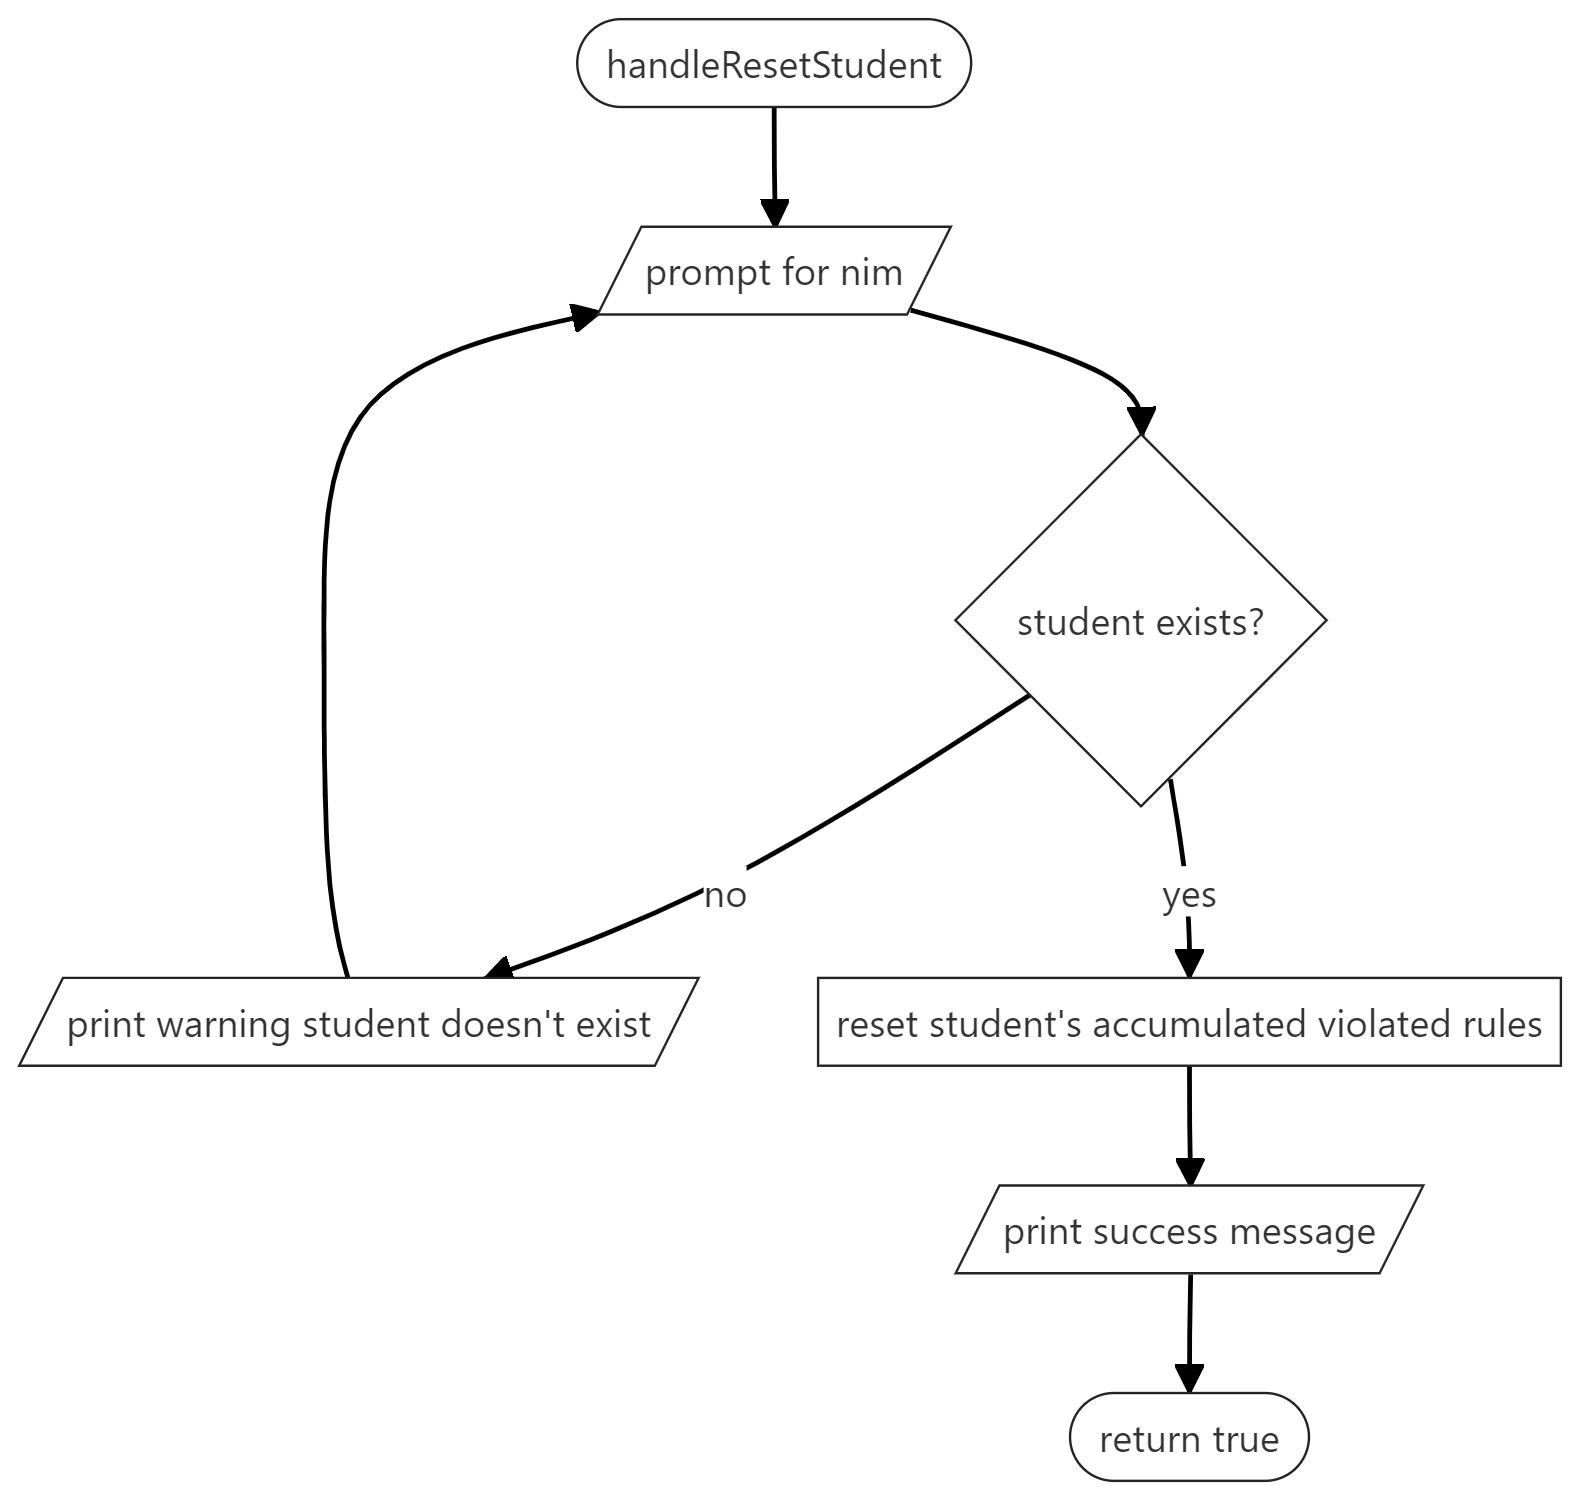
\includegraphics[width=8cm]{flowcharts/handle-reset-student.png}
    \caption{\texttt{handleResetStudent()}}
\end{figure}

\pagebreak

\subsection{Rule Menu}

\begin{figure}[h]
    \centering
    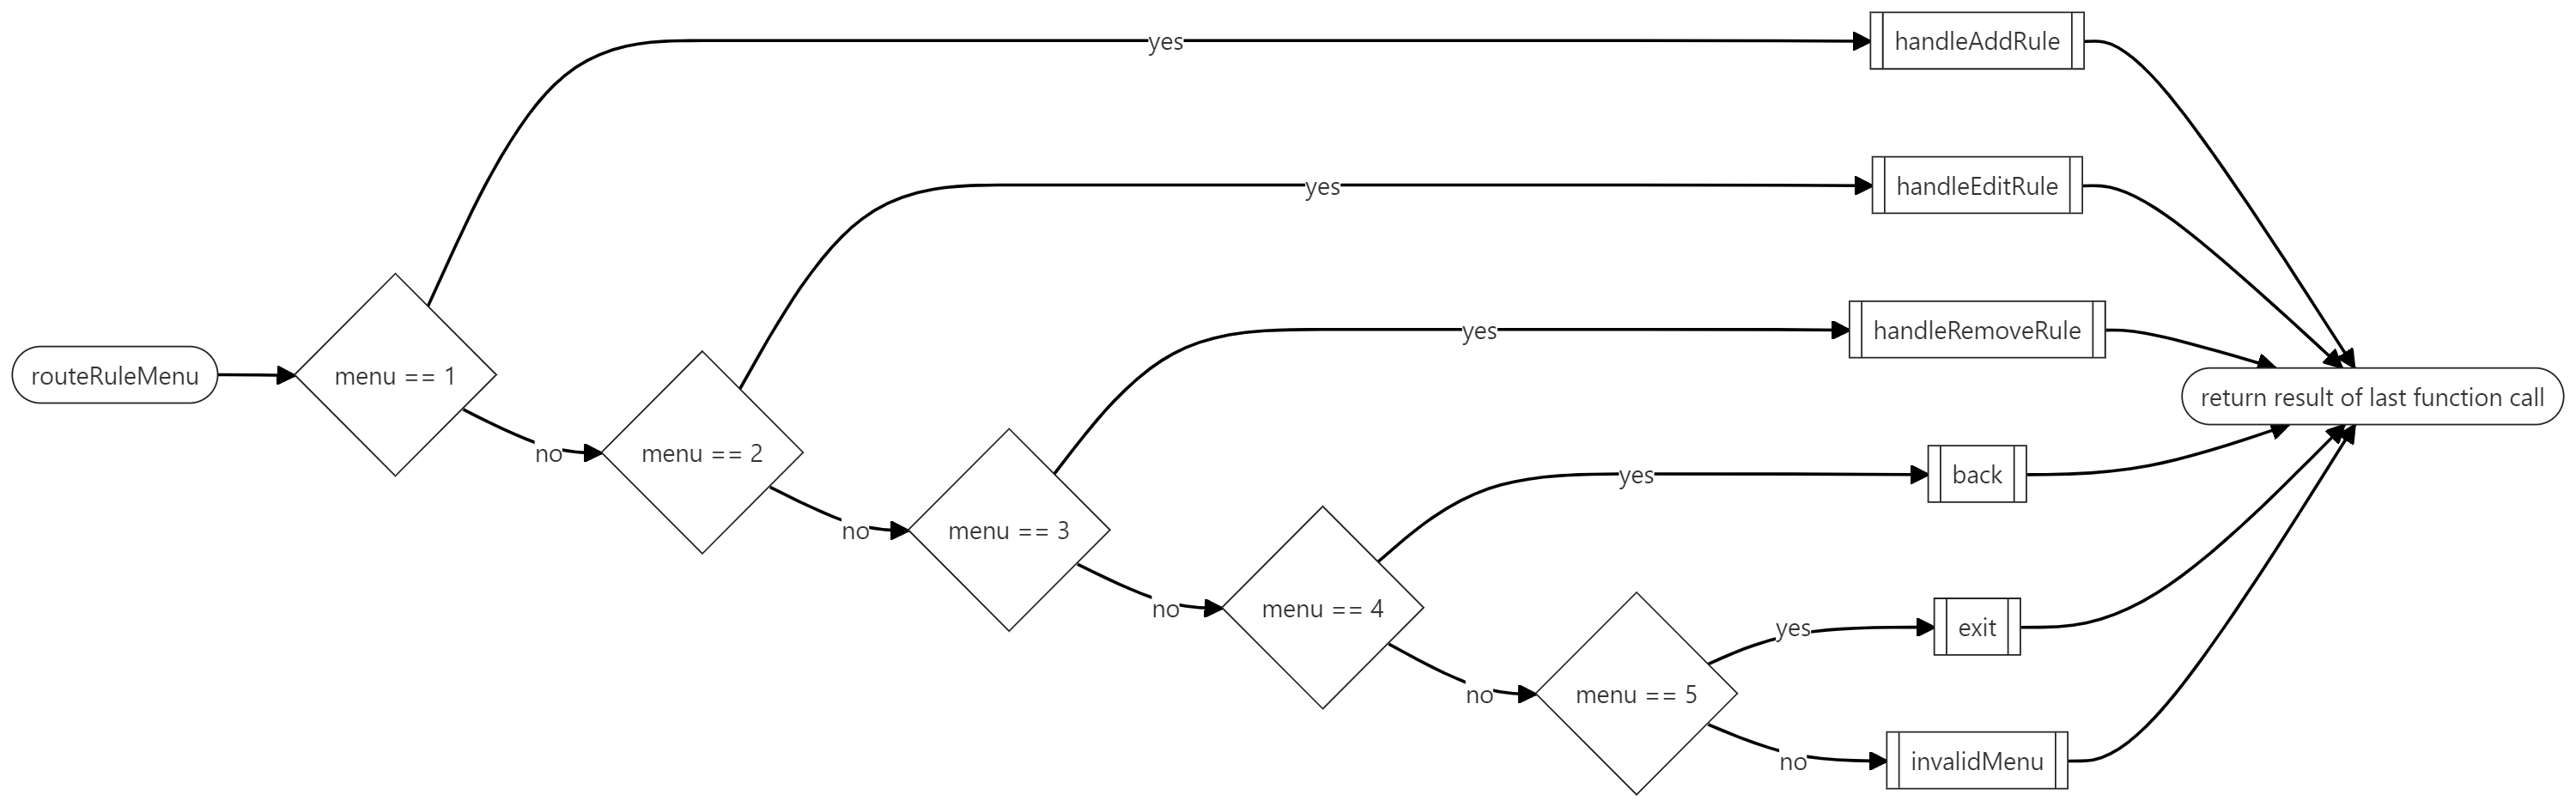
\includegraphics[width=\textwidth]{flowcharts/route-rule-menu.png}
    \caption{\texttt{routeRuleMenu()}}
\end{figure}

\pagebreak

\begin{figure}[h]
    \centering
    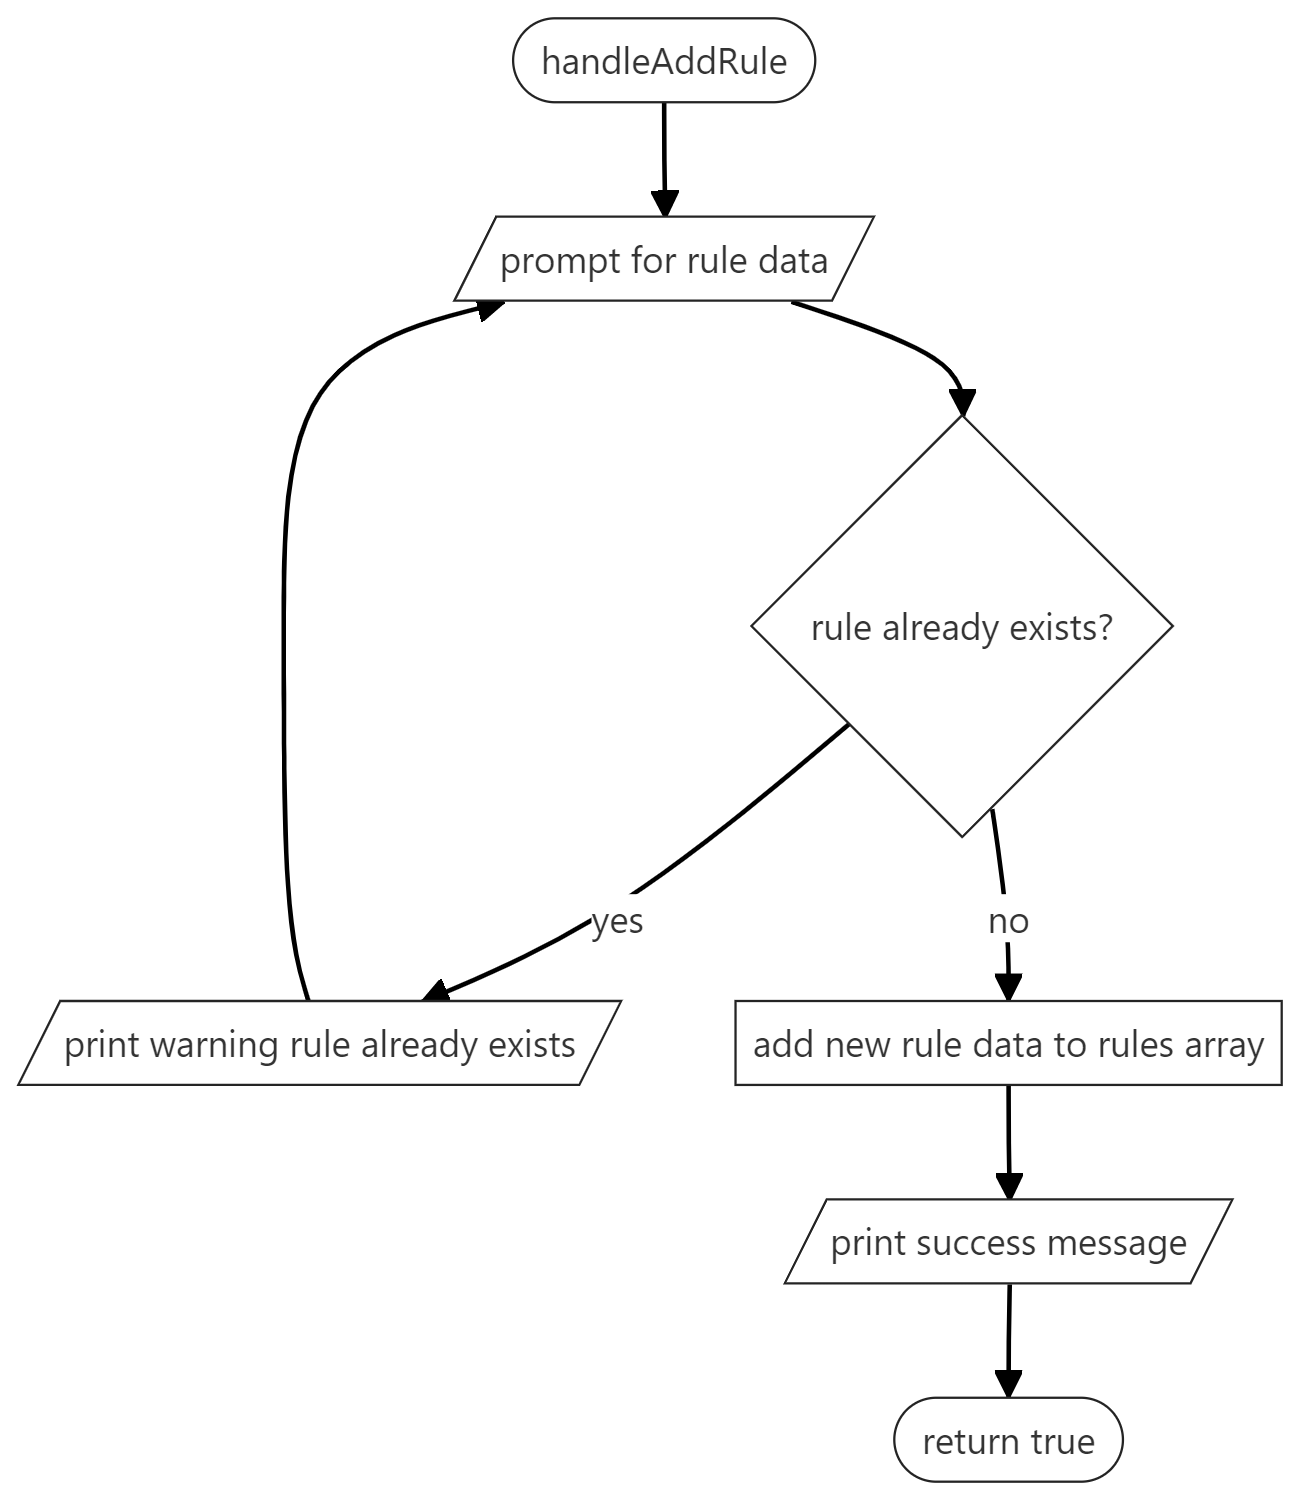
\includegraphics[height=7.2cm]{flowcharts/handle-add-rule.png}
    \caption{\texttt{handleAddRule()}}
\end{figure}

\begin{figure}[h]
    \centering
    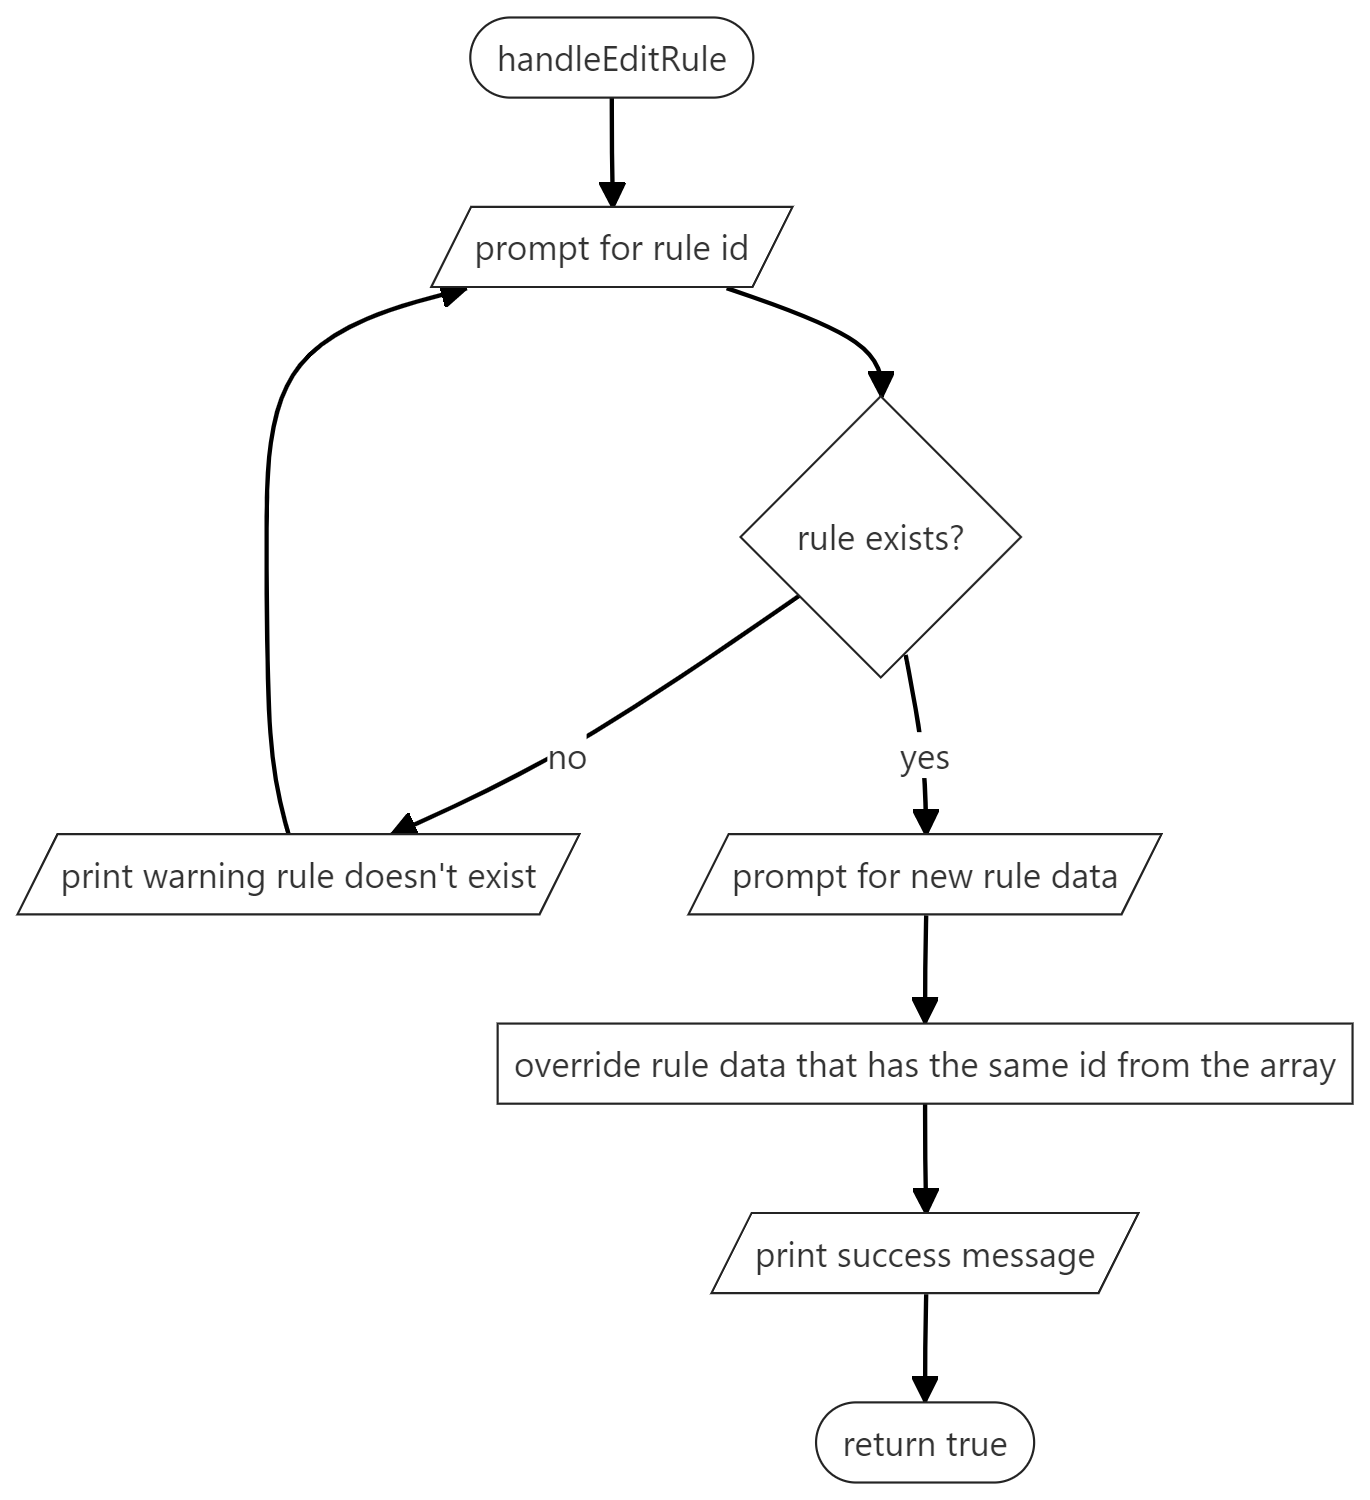
\includegraphics[height=7.2cm]{flowcharts/handle-edit-rule.png}
    \caption{\texttt{handleEditRule()}}
\end{figure}

\pagebreak

\begin{figure}[h]
    \centering
    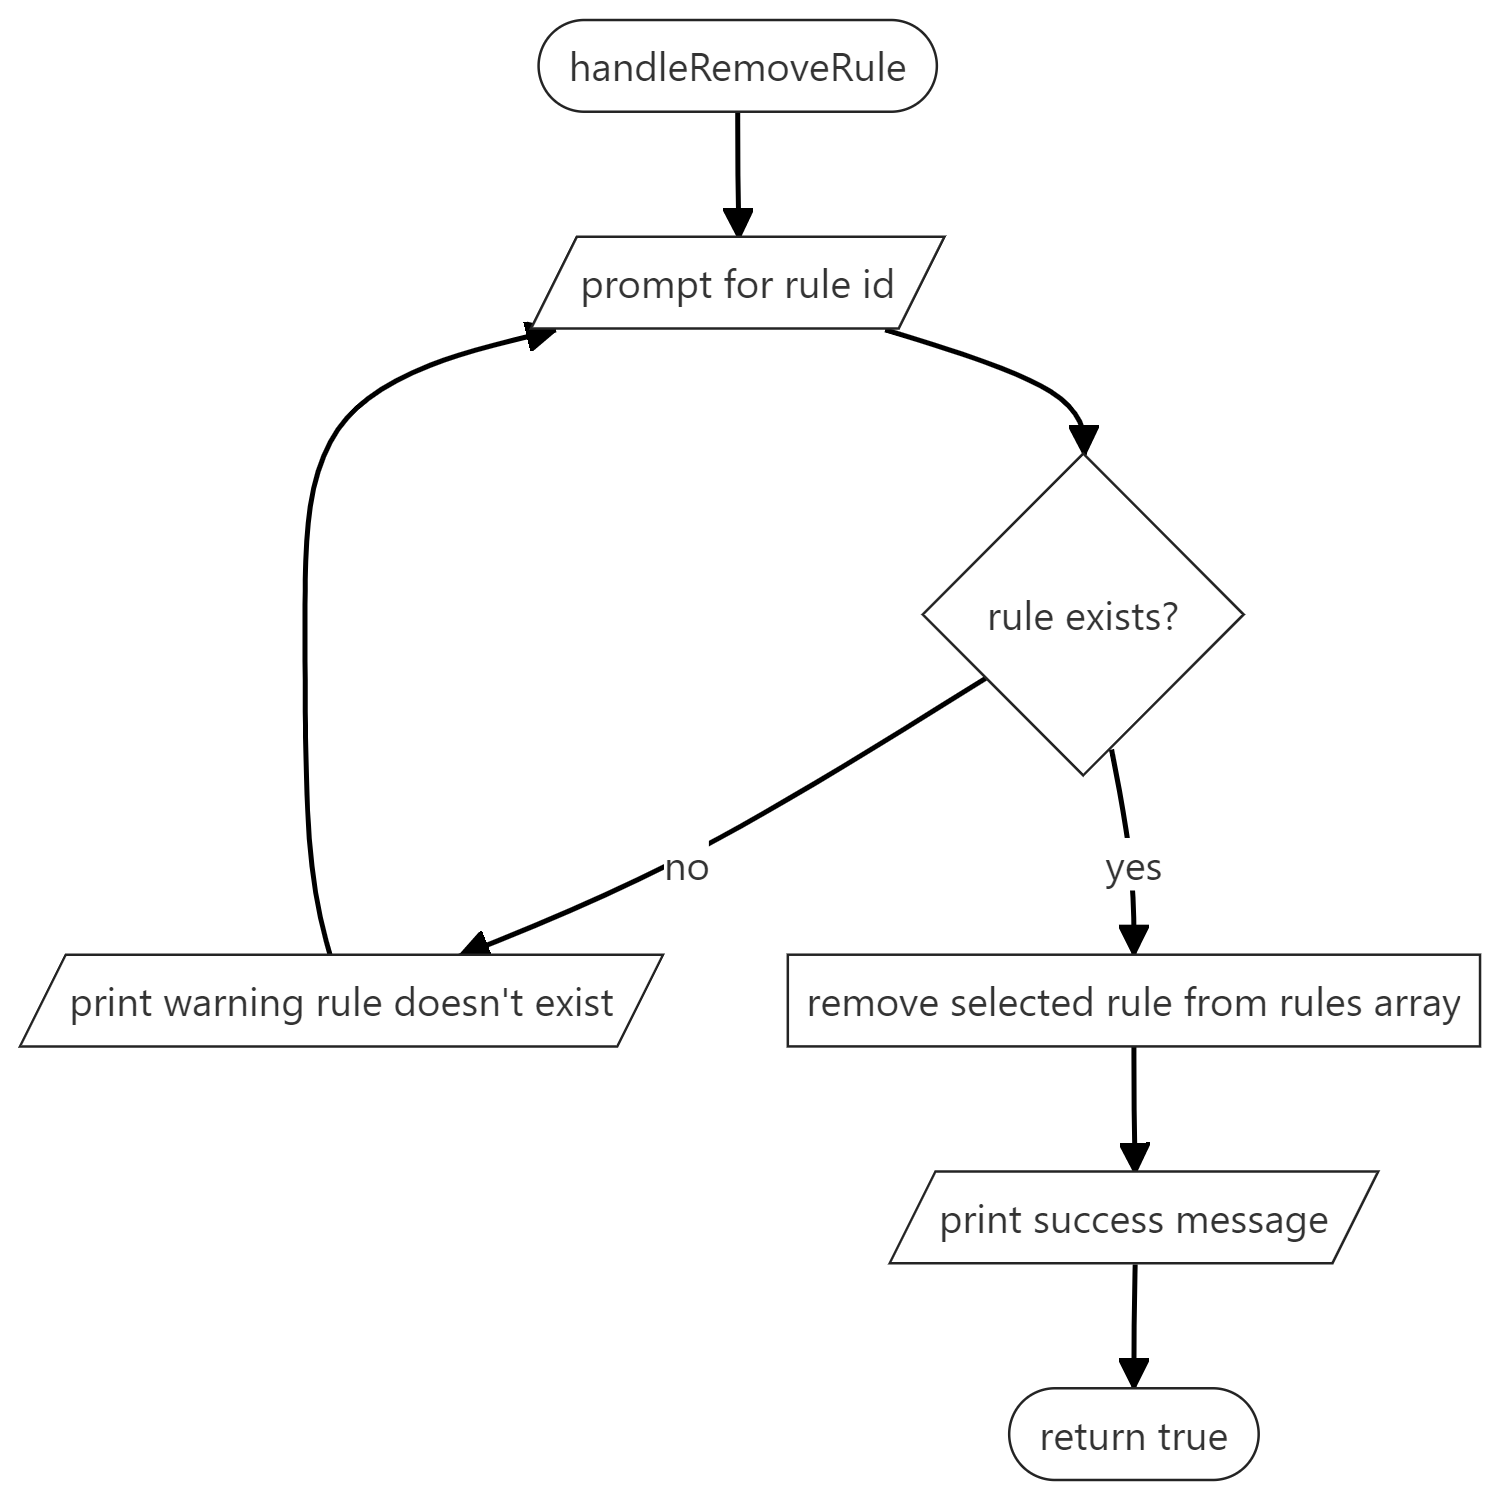
\includegraphics[width=7.2cm]{flowcharts/handle-remove-rule.png}
    \caption{\texttt{handleRemoveRule()}}
\end{figure}

\pagebreak

\section{Code}

\begin{minted}[linenos,autogobble,breaklines,fontsize=\footnotesize]{java}
package my.id.elianiva; // remove this to run on a single file mode

import java.util.Scanner;

public class Main {
    static String LINE_PLUS = "+";
    static String LINE_HORIZONTAL = "-";
    static String LINE_VERTICAL = "|";
    static String USERNAME = "admin";
    static String PASSWORD = "admin123";

    // [nim, fullName, classPlacement, violatedRuleIndices, currentPunishment, violationsCount]
    static String[][] students = {
            {"1234560001", "Harimurti Suryono", "1A", "", "", "0"},
            {"1234560002", "Carla Andriani", "1B", "", "", "0"},
            {"1234560003", "Hana Astuti", "1C", "", "", "0"},
            {"1234560004", "Rini Padmasari", "1D", "", "", "0"},
            {"1234560005", "Karsana Nababan", "1E", "", "", "0"}
    };

    // [code, description, level]
    static String[][] rules = {
            {"R001", "Communicating in a disrespectful manner, whether written or written to students, lecturers, employees, or others", "5"},
            {"R002", "Eating, or drinking in the lecture theatre/laboratory/workshop", "4"},
            {"R003", "Students sporting punk-style hair, painted other than black and/or skinned", "4"},
            {"R004", "Violating the rules / regulations that apply in Polinema both in the Department / Study Programme", "3"},
            {"R005", "Not maintaining cleanliness in all areas of Polinema", "3"},
            {"R006", "Smoking outside the smoking area", "3"},
            {"R007", "Playing cards, online games in the campus area", "3"},
            {"R008", "Damaging facilities and infrastructure in the Polinema area", "2"},
            {"R009", "Accessing pornographic material in class or campus areas", "2"},
            {"R010", "Conducting practical political activities on campus", "2"},
            {"R012", "Using psychotropic substances and / or other addictive substances other addictive substances", "1"},
    };

    static String[] punishments = {
            "Oral reprimand accompanied by a statement not to repeat the act, affixed with stamp duty, signed by the student concerned and DPA",
            "A written reprimand accompanied by a statement not to repeat the act, affixed with a stamp duty",
            """
               a. Make a statement not to repeat the act, affixed with stamp duty, signed by the student concerned and DPA
                    b. Perform special tasks, such as being responsible for repairing or cleaning up, and other tasks. cleaning, and other tasks.""",
            """
                a. Compensation for damages or replacement of similar objects/goods and/or
                     b. Performing social service duties for a certain period of time and/or
                     c. Given a grade of D in the relevant course when committing the offence""",
            """
                a. Disabled (Academic/Terminal Leave) for two semesters and/or
                     b. Dismissed as a student."""
    };

    static Scanner scanner = new Scanner(System.in);

    public static void main(String[] args) {
        clearScreen();
        renderTitle("Welcome! Please log in first!");
        login();
        clearScreen();
        renderTitle("Welcome back, " + USERNAME);
        while (true) {
            renderTitle("MAIN MENU");
            int chosenMenu = pickMenu("Main Menu: ", new String[]{
                    "Show Students",
                    "Show Rules",
                    "Exit"
            });
            boolean shouldContinue = routeMainMenu(chosenMenu);
            if (shouldContinue) continue;
            break;
        }
    }

    static void login() {
        while (true) {
            String username = getNonEmptyString("Username: ", "Username can't be empty!");
            String password = getNonEmptyString("Password: ", "Password can't be empty!");
            if (username.equals(USERNAME) && password.equals(PASSWORD)) {
                break;
            }
            clearScreen();
            System.out.println("Incorrect username and password!");
        }
    }

    static boolean routeMainMenu(int chosenMenu) {
        return switch (chosenMenu) {
            case 1 -> handleShowStudents();
            case 2 -> handleShowRules();
            case 3 -> exit();
            default -> handleInvalidMenu();
        };
    }

    static boolean routeStudentMenu(int chosenMenu) {
        return switch (chosenMenu) {
            case 1 -> handleShowStudentDetail();
            case 2 -> handleAddViolatedRuleToStudent();
            case 3 -> handleAddStudent();
            case 4 -> handleEditStudent();
            case 5 -> handleRemoveStudent();
            case 6 -> handleResetStudent();
            case 7 -> back();
            case 8 -> exit();
            default -> handleInvalidMenu();
        };
    }

    static boolean routeRuleMenu(int chosenMenu) {
        return switch (chosenMenu) {
            case 1 -> handleAddRule();
            case 2 -> handleEditRule();
            case 3 -> handleRemoveRule();
            case 4 -> back();
            case 5 -> exit();
            default -> handleInvalidMenu();
        };
    }

    static boolean exit() {
        clearScreen();
        renderTitle("Exiting...");
        System.exit(0);
        return false;
    }

    static boolean back() {
        clearScreen();
        return false;
    }

    static boolean handleInvalidMenu() {
        System.out.println("Invalid menu!");
        clearScreen();
        return true;
    }

    static boolean handleShowStudents() {
        clearScreen();
        while (true) {
            renderStudentsTable("Showing All Students", students);
            int chosenMenu = pickMenu("Students Table Menu: ", new String[]{
                    "Show Student Detail",
                    "Add Student Violated Rule",
                    "Add Student",
                    "Edit Student",
                    "Remove Student",
                    "Reset Student",
                    "Back",
                    "Exit",
            });
            boolean shouldContinue = routeStudentMenu(chosenMenu);
            if (shouldContinue) continue;
            break;
        }
        return true;
    }

    static boolean handleShowStudentDetail() {
        clearScreen();
        String nim;

        while (true) {
            renderTitle("Select Student");
            renderStudentsTable("Showing All Students", students);
            nim = getNonEmptyString("NIM: ", "NIM can't be empty!");

            if (has(students, nim, 0)) break;

            clearScreen();
            System.out.println("Student with the NIM of " + nim + " doesn't exist!");
        }

        clearScreen();
        renderTitle("Showing Details for Student " + nim);

        int studentIndex = -1;
        for (int i = 0; i < students.length; i++) {
            if (students[i][0].equals(nim)) {
                studentIndex = i;
                break;
            }
        }
        if (studentIndex == -1) {
            clearScreen();
            System.out.println("Failed to find the student with a nim of " + nim);
            return true;
        }

        String[] student = students[studentIndex];
        System.out.println("NIM\t\t: " + student[0]);
        System.out.println("Name\t\t: " + student[1]);
        System.out.println("Class\t\t: " + student[2]);

        if (student[3].length() > 0) {
            renderRulesTable("Rules that have been violated", filterRulesByIndices(rules, student[3]));
        }

        if (student[4].length() > 0) {
            renderPunishmentsList("Punishments", filterPunishmentsByIndices(punishments, student[4]));
        }

        getString("Press enter to continue...");

        clearScreen();
        return true;
    }

    static boolean handleAddViolatedRuleToStudent() {
        clearScreen();
        String nim, code;

        int studentIndex = -1;
        while (true) {
            renderTitle("Add Violated Rule to Student");
            renderStudentsTable("Showing All Students", students);
            nim = getNonEmptyStringWithLimit("Student's NIM: ", "NIM can't be empty!", 10, 10, false);

            if (!has(students, nim, 0)) {
                clearScreen();
                System.out.println("Student with the NIM of " + nim + " doesn't exist!");
                continue;
            }

            for (int i = 0; i < students.length; i++) {
                if (students[i][0].equals(nim)) {
                    studentIndex = i;
                    break;
                }
            }

            if (students[studentIndex][3].length() == 3) {
                System.out.println("This student has maxed out the violated rule limit.");
                System.out.println("Please make sure the student has done the punishments and reset the data after that.");
                getString("Press enter to continue...");
                return true;
            }

            break;
        }

        clearScreen();

        int ruleIndex = -1;
        while (true) {
            renderTitle("Add Violated Rule to Student");
            renderRulesTable("Showing All Rules", rules);
            code = getNonEmptyStringWithLimit("Rule's Code: ", "Code can't be empty!", 4, 4, false);

            if (!has(rules, code, 0)) {
                clearScreen();
                System.out.println("Rule with the code of " + code + " doesn't exist!");
                continue;
            }

            for (int i = 0; i < rules.length; i++) {
                if (rules[i][0].equals(code)) {
                    ruleIndex = i;
                    break;
                }
            }

            break;
        }

        String[] currentStudent = students[studentIndex];

        boolean isUpgraded = shouldUpgrade(currentStudent, rules[ruleIndex]);
        currentStudent[3] += toString(ruleIndex);
        currentStudent[4] += resolvePunishmentIndex(currentStudent[3], isUpgraded);
        currentStudent[5] = incrementString(currentStudent[5], Integer.MAX_VALUE);

        clearScreen();
        System.out.println("Rule have been added to the student successfully");

        return true;
    }

    static boolean handleAddStudent() {
        clearScreen();
        String nim, fullName, classPlacement;

        while (true) {
            renderTitle("Add New Student");
            nim = getNonEmptyStringWithLimit("NIM: ", "NIM can't be empty!", 10, 10, false);
            fullName = getNonEmptyStringWithLimit("Full Name: ", "Full Name can't be empty!", 1, 20, false);
            classPlacement = getNonEmptyStringWithLimit("Class: ", "Class can't be empty!", 1, 2, false);

            if (!has(students, nim, 0)) break;

            clearScreen();
            System.out.println("Student with the NIM of " + nim + " already exists!");
        }

        String[][] newStudents = new String[students.length + 1][2];
        for (int i = 0; i < students.length; i++) {
            newStudents[i] = students[i];
        }
        newStudents[newStudents.length - 1] = new String[]{nim, fullName, classPlacement, "", "", "0"};
        students = newStudents;

        clearScreen();
        System.out.println("Students have been succesfully added!");
        return true;
    }

    static boolean handleEditStudent() {
        clearScreen();
        String oldNim, nim, fullName, classPlacement;
        int studentIndex = -1;

        while (true) {
            renderTitle("Edit Student");
            renderStudentsTable("Showing Students to Edit", students);
            oldNim = getNonEmptyStringWithLimit("NIM: ", "NIM can't be empty!", 10, 10, false);

            if (has(students, oldNim, 0)) break;

            clearScreen();
            System.out.println("The student with the NIM of " + oldNim + " doesn't exists");
        }

        for (int i = 0; i < students.length; i++) {
            if (students[i][0].equals(oldNim)) {
                studentIndex = i;
                break;
            }
        }

        if (studentIndex == -1) {
            clearScreen();
            System.out.println("Failed to find student to edit");
            return true;
        }

        String[] student = students[studentIndex];

        clearScreen();
        renderTitle("New Student Data");
        nim = getNonEmptyStringWithLimit("NIM (old: " + student[0] + "): ", "NIM can't be empty!", 10, 10, true);
        fullName = getNonEmptyStringWithLimit("Full Name (old: " + student[1] + "): ", "Full Name can't be empty!", 1, 20, true);
        classPlacement = getNonEmptyStringWithLimit("Class (old: " + student[2] + "): ", "Class can't be empty!", 1, 2, true);

        students[studentIndex][0] = nim.isEmpty() ? student[0] : nim;
        students[studentIndex][1] = fullName.isEmpty() ? student[1] : fullName;
        students[studentIndex][2] = classPlacement.isEmpty() ? student[2] : classPlacement;

        clearScreen();
        System.out.println("Students have been succesfully added!");
        return true;
    }

    static boolean handleRemoveStudent() {
        clearScreen();
        String nim;

        while (true) {
            renderTitle("Remove Student");
            renderStudentsTable("Showing Students to Remove", students);
            nim = getNonEmptyString("NIM: ", "NIM can't be empty!");

            if (has(students, nim, 0)) break;

            clearScreen();
            System.out.println("Student with the NIM of " + nim + " doesn't exist!");
        }

        String[][] filteredStudents = new String[students.length - 1][4];
        int count = 0;
        for (String[] student : students) {
            if (student[0].equals(nim)) continue;
            filteredStudents[count] = student;
            count++;
        }
        students = filteredStudents;

        clearScreen();
        System.out.println("Students " + nim + " have been successfully removed!");
        return true;
    }

    static boolean handleResetStudent() {
        clearScreen();
        String nim;


        int studentIndex = -1;
        while (true) {
            renderTitle("Reset Student");
            renderStudentsTable("Showing Students to Reset", students);
            nim = getNonEmptyStringWithLimit("Student's NIM: ", "NIM can't be empty!", 10, 10, false);

            if (!has(students, nim, 0)) {
                clearScreen();
                System.out.println("Student with the NIM of " + nim + " doesn't exist!");
                continue;
            }

            for (int i = 0; i < students.length; i++) {
                if (students[i][0].equals(nim)) {
                    studentIndex = i;
                    break;
                }
            }

            break;
        }

        students[studentIndex][3] = "";
        students[studentIndex][4] = "";

        clearScreen();
        System.out.println("Students have been successfully reset!");
        return true;
    }

    static boolean handleShowRules() {
        clearScreen();
        while (true) {
            renderRulesTable("Showing All Rules", rules);
            int chosenMenu = pickMenu("Rules Table Menu: ", new String[]{
                    "Add Rule",
                    "Edit Rule",
                    "Remove Rule",
                    "Back",
                    "Exit",
            });
            boolean shouldContinue = routeRuleMenu(chosenMenu);
            if (shouldContinue) continue;
            break;
        }
        return true;
    }

    static boolean handleAddRule() {
        clearScreen();
        String code, description;
        int level;

        while (true) {
            renderTitle("Add New Rule");
            code = getNonEmptyStringWithLimit("Code: ", "Code can't be empty!", 4, 4, false);
            description = getNonEmptyStringWithLimit("Description: ", "Description can't be empty!", 10, 120, false);
            level = getIntegerWithRange("Level: ", 1, 5, false);

            if (!has(rules, code, 0)) break;

            clearScreen();
            System.out.println("Rule with the code of " + code + " already exists!");
        }

        String[][] newRules = new String[rules.length + 1][2];
        for (int i = 0; i < rules.length; i++) {
            newRules[i] = rules[i];
        }
        newRules[newRules.length - 1] = new String[]{code, description, toString(level)};
        rules = newRules;

        clearScreen();
        System.out.println("New rule have been successfully added!");
        return true;
    }

    static boolean handleEditRule() {
        clearScreen();
        String oldCode, code, description;
        int level;
        int ruleIndex = -1;

        while (true) {
            renderTitle("Edit Rule");
            renderRulesTable("Showing Rules to Edit", rules);
            oldCode = getNonEmptyStringWithLimit("Code: ", "Code can't be empty!", 4, 4, false);

            if (has(rules, oldCode, 0)) break;

            clearScreen();
            System.out.println("The rule with the code of " + oldCode + " doesn't exists");
        }

        for (int i = 0; i < rules.length; i++) {
            if (rules[i][0].equals(oldCode)) {
                ruleIndex = i;
                break;
            }
        }

        if (ruleIndex == -1) {
            clearScreen();
            System.out.println("Failed to find rule to edit");
            return true;
        }

        String[] rule = rules[ruleIndex];

        clearScreen();
        renderTitle("New Rule Detail");
        while (true) {
            code = getNonEmptyStringWithLimit("Code (old: " + rule[0] + "): ", "Code can't be empty!", 4, 4, true);
            if (!has(rules, code, 0)) break;
            System.out.println("There's a rule with the same code already! Please try another one.");
        }
        description = getNonEmptyStringWithLimit("Description (old: " + rule[1] + "): ", "Description can't be empty!", 10, 120, true);
        level = getIntegerWithRange("Level (old: " + rule[2] + "): ", 1, 5, true);

        rules[ruleIndex][0] = code.isEmpty() ? rule[0] : code;
        rules[ruleIndex][1] = description.isEmpty() ? rule[1] : description;
        rules[ruleIndex][2] = level == -1 ? rule[2] : String.format("%s", level);

        clearScreen();
        System.out.println("Rule " + oldCode + " have been succesfully edited!");
        return true;
    }

    static boolean handleRemoveRule() {
        clearScreen();
        String code;

        while (true) {
            renderTitle("Remove Rule");
            renderRulesTable("Showing Rules to Remove", rules);
            code = getNonEmptyString("Code: ", "Code can't be empty!");

            if (has(rules, code, 0)) break;

            clearScreen();
            System.out.println("Rule with the code of " + code + " doesn't exist!");
        }

        String[][] filteredRules = new String[rules.length - 1][3];
        int count = 0;
        for (int i = 0; i < rules.length; i++) {
            if (rules[i][0].equals(code)) continue;
            filteredRules[count] = rules[i];
            count++;
        }
        rules = filteredRules;

        clearScreen();
        System.out.println("Rule " + code + " have been successfully removed!");
        return true;
    }

    static void renderTitle(String title) {
        int paddingSize = 4;
        int titleLength = title.length();

        String horizontalBorder = LINE_PLUS + LINE_HORIZONTAL.repeat(titleLength + paddingSize * 2) + LINE_PLUS;

        System.out.println(horizontalBorder);
        System.out.println(LINE_VERTICAL + " ".repeat(paddingSize) + title + " ".repeat(paddingSize) + LINE_VERTICAL);
        System.out.println(horizontalBorder);
    }

    static void renderStudentsTable(String title, String[][] students) {
        renderTitle(title);
        final String tableLine = String.format(
                "%s%s%s%s%s%s%s%s%s%s%s",
                LINE_PLUS, LINE_HORIZONTAL.repeat(6), LINE_PLUS, LINE_HORIZONTAL.repeat(14),
                LINE_PLUS, LINE_HORIZONTAL.repeat(24), LINE_PLUS, LINE_HORIZONTAL.repeat(9),
                LINE_PLUS, LINE_HORIZONTAL.repeat(14), LINE_PLUS
        );
        System.out.println(tableLine);
        System.out.printf("%s  No. %s     NIM      %s       Full Name        %s  Class  %s  Violations  %s\n", LINE_VERTICAL, LINE_VERTICAL, LINE_VERTICAL, LINE_VERTICAL, LINE_VERTICAL, LINE_VERTICAL);
        System.out.println(tableLine);
        for (int i = 0; i < students.length; i++) {
            String[] student = students[i];
            System.out.printf(
                    "%s  %-2s  %s  %-10s  %s  %-20s  %s  %5s  %s   %8s   %s\n",
                    LINE_VERTICAL, (i + 1) + ".", LINE_VERTICAL, student[0], LINE_VERTICAL, student[1],
                    LINE_VERTICAL, student[2], LINE_VERTICAL, student[5], LINE_VERTICAL);
        }
        System.out.println(tableLine);
    }

    static void renderRulesTable(String title, String[][] rules) {
        renderTitle(title);
        final String tableLine = String.format(
                "%s%s%s%s%s%s%s%s%s",
                LINE_PLUS, LINE_HORIZONTAL.repeat(7), LINE_PLUS, LINE_HORIZONTAL.repeat(10),
                LINE_PLUS, LINE_HORIZONTAL.repeat(124), LINE_PLUS, LINE_HORIZONTAL.repeat(9), LINE_PLUS);
        System.out.println(tableLine);
        System.out.printf(
                "%s  No.  %s    ID    %s  %sDescription%s   %s  Level  %s\n",
                LINE_VERTICAL, LINE_VERTICAL, LINE_VERTICAL, " ".repeat(54), " ".repeat(54), LINE_VERTICAL, LINE_VERTICAL);
        System.out.println(tableLine);
        for (int i = 0; i < rules.length; i++) {
            String[] rule = rules[i];
            System.out.printf(
                    "%s  %3s  %s   %-5s  %s  %-120s  %s  %5s  %s\n",
                    LINE_VERTICAL, (i + 1) + ".", LINE_VERTICAL, rule[0], LINE_VERTICAL, rule[1],
                    LINE_VERTICAL, rule[2], LINE_VERTICAL);
        }
        System.out.println(tableLine);
    }

    static void renderPunishmentsList(String title, String[] punishments) {
        renderTitle(title);
        for (int i = 0; i < punishments.length; i++) {
            String punishment = punishments[i];
            System.out.printf("%3s  %-120s\n", (i + 1) + ".)", punishment);
        }
    }

    static int pickMenu(String menuTitle, String[] menus) {
        System.out.println(menuTitle);
        for (int i = 0; i < menus.length; i++) {
            System.out.printf("%d. %s\n", i + 1, menus[i]);
        }
        return getIntegerWithRange("Select menu: ", 1, menus.length, false);
    }

    static String getString(String prompt) {
        System.out.print(prompt);
        return scanner.nextLine().trim();
    }

    static String getNonEmptyString(String prompt, String warning) {
        while (true) {
            System.out.print(prompt);
            String userInput = scanner.nextLine().trim();
            if (!userInput.isEmpty()) return userInput;
            System.out.println(warning);
        }
    }

    static String getNonEmptyStringWithLimit(String prompt, String warning, int min, int max, boolean allowEmpty) {
        while (true) {
            String userInput = allowEmpty ? getString(prompt) : getNonEmptyString(prompt, warning);
            if (allowEmpty && userInput.isEmpty()) return userInput;
            if (userInput.length() >= min && userInput.length() <= max) return userInput;
            System.out.println("The input can't be shorter than " + min + " or longer than " + max);
        }
    }

    static int getIntegerWithRange(String prompt, int min, int max, boolean allowEmpty) {
        while (true) {
            System.out.print(prompt);
            String userInputStr = scanner.nextLine();
            if (userInputStr.isEmpty()) {
                if (allowEmpty) return -1;
                System.out.println("Input can't be empty!");
                continue;
            }

            int userInput = Integer.parseInt(userInputStr);
            if (userInput >= min && userInput <= max) return userInput;

            System.out.println("The input can't be lower than " + min + " or greater than " + max);
        }
    }

    static void clearScreen() {
        System.out.print("\033[H\033[2J");
        System.out.flush();
    }

    static boolean has(String[][] items, String needle, int fieldIndex) {
        for (String[] item : items) {
            if (item[fieldIndex].equals(needle)) return true;
        }
        return false;
    }

    static String toString(int number) {
        return String.format("%d", number);
    }

    static String toString(char character) {
        return String.format("%c", character);
    }

    static boolean shouldUpgrade(String[] student, String[] nextRule) {
        String ruleIndices = student[3];
        int length = ruleIndices.length();
        if (length < 2) return false;

        boolean lastThreeRuleAreSame = true;
        String previousLevel = "";
        for (int i = length - 1; i > length - 3; i--) {
            String[] currentRule = rules[Integer.parseInt(toString(ruleIndices.charAt(i)))];
            if (!previousLevel.isEmpty() && !currentRule[2].equals(previousLevel)) {
                lastThreeRuleAreSame = false;
                break;
            }
            previousLevel = currentRule[2];
        }
        if (!previousLevel.equals(nextRule[2])) {
            lastThreeRuleAreSame = false;
        }

        return lastThreeRuleAreSame;
    }

    static String incrementString(String previous, int limit) {
        int prev = Integer.parseInt(previous);
        int now = prev + 1;
        return now < limit ? toString(now) : previous;
    }

    static String resolvePunishmentIndex(String currentLevel, boolean isUpgraded) {
        int lastRuleIndex = Integer.parseInt(toString(currentLevel.charAt(currentLevel.length() - 1)));
        int lastLevel = Integer.parseInt(rules[lastRuleIndex][2]);

        if (!isUpgraded || lastLevel == 1) return toString(punishments.length - lastLevel);

        return toString(punishments.length - (lastLevel - 1));
    }

    static String[][] filterRulesByIndices(String[][] rules, String indices) {
        String[][] filteredRules = new String[indices.length()][3];
        for (int i = 0; i < indices.length(); i++) {
            int index = Integer.parseInt(String.format("%c", indices.charAt(i)));
            filteredRules[i] = rules[index];
        }
        return filteredRules;
    }

    static String[] filterPunishmentsByIndices(String[] punishments, String indices) {
        String[] filteredPunishments = new String[indices.length()];
        for (int i = 0; i < indices.length(); i++) {
            int index = Integer.parseInt(String.format("%c", indices.charAt(i)));
            filteredPunishments[i] = punishments[index];
        }
        return filteredPunishments;
    }
}
\end{minted}

\end{document}

